\documentclass[12pt,a4paper, twoside]{book}
\usepackage[latin1]{inputenc} 
\usepackage[T1]{fontenc} 
\usepackage{graphicx} 
\usepackage{amsmath,amssymb}
\usepackage{color}
\usepackage{listings}
\usepackage[pdftex,colorlinks=true,bookmarks=true, linkcolor=blue]{hyperref}
\lstset{language=c++}
\lstset{basicstyle=\small}
\lstset{backgroundcolor=\color{white}}
\lstset{frame=single}
\lstset{stringstyle=\ttfamily}
\lstset{keywordstyle=\color{red}\bfseries}
\lstset{commentstyle=\itshape\color{blue}}
\lstset{showspaces=false}
\lstset{showstringspaces=false}
\lstset{showtabs=false}
\lstset{breaklines}
 
\newcommand{\be}{\begin{equation}}
\newcommand{\bes}{\begin{equation*}}
\newcommand{\bea}{\begin{eqnarray}}
\newcommand{\beas}{\begin{eqnarray*}}

\newcommand{\bml}{\begin{multline}}
\newcommand{\eml}{\end{multline}}

\newcommand{\bs}{\begin{split}}
\newcommand{\es}{\end{split}}

\newcommand{\bi}{\begin{itemize}}
\newcommand{\ei}{\end{itemize}}

\newcommand{\ee}{\end{equation}}
\newcommand{\ees}{\end{equation*}}
\newcommand{\eea}{\end{eqnarray}}
\newcommand{\eeas}{\end{eqnarray*}}

\newcommand{\dd}[1]{\frac{d^2}{d {#1}^2}}
\newcommand{\ddf}[2]{\frac{d^2 #1}{d {#2}^2}}

\newcommand{\sd}[1]{\frac{d}{d {#1}}}

\newcommand{\deriv}[2]{\frac{d{#1}}{d {#2}}}
\newcommand{\pd}[1]{\frac{\partial {}}{\partial {#1}}}
\newcommand{\pdd}[1]{\frac{\partial^2 {}}{\partial {#1^2}}}
\newcommand{\pdn}[1]{\frac{\partial^n {}}{\partial {#1^n}}}
\newcommand{\pdnm}[2]{\frac{\partial^{#1} {}}{\partial {#2^{#1}}}}
\newcommand{\pdf}[2]{\frac{\partial {#1}}{\partial {#2}}}
\newcommand{\pdff}[2]{\frac{\partial^2 {#1}}{\partial {#2^2}}}
\newcommand{\pdfn}[3]{\frac{\partial^#1 {#2}}{\partial {#3^#1}}}

\newcommand{\f}[1]{\boldsymbol{#1}}
\newcommand{\mmbf}[1]{$\mathbf{#1}$}
\newcommand{\mbf}[1]{\mathbf{#1}}

\newcommand{\mmxtp}{\mmbf{X_T}}
\newcommand{\mxtp}{\mbf{X_T}}

\newcommand{\psiij}{\psi_{ij}}
\newcommand{\psiji}{\psi_{ji}}

\newcommand{\psisd}{\psi_{SD}}
\newcommand{\psisdx}{\psi_{SD}(\f x)}
\newcommand{\psisdy}{\psi_{SD}(\f y)}

\newcommand{\psisdu}{\psi_{SD\uparrow}}
\newcommand{\psisdux}{\psi_{SD\uparrow}(\f x)}
\newcommand{\psisduy}{\psi_{SD\uparrow}(\f y)}
\newcommand{\psisdd}{\psi_{SD\downarrow}}
\newcommand{\psisddx}{\psi_{SD\downarrow}(\f x)}
\newcommand{\psisddy}{\psi_{SD\downarrow}(\f y)}

\newcommand{\varparam}{\f \alpha}
\newcommand{\PsiTrial}{\Psi_{\varparam}}

\newcommand{\delratio}[1]{ \frac{\nabla_k \psisd (\f #1)}{\psisd (\f #1)} }
\newcommand{\ratio}{\frac{\psisdx}{\psisdy}}
\newcommand{\ratioup}{\frac{\psisdx}{\psisdy}}
\newcommand{\delsqratio}[1]{ \frac{\nabla_k^2 \psisd (\f #1)}{\psisd (\f #1)} }

\newcommand{\sminv}{S^{-1}}
\newcommand{\detsm}{|S|}
\newcommand{\detsmx}{|S(\f x)|}
\newcommand{\detsmy}{|S(\f y)|}

\newcommand{\rij}{r_{ij}}
\newcommand{\rijvec}{\f r_{ij}}
\newcommand{\rikvec}{\f r_{ik}}
\newcommand{\rkivec}{\f r_{ki}}

\newcommand{\rkj}{r_{kj}}
\newcommand{\rik}{r_{ik}}
\newcommand{\rki}{r_{ki}}

\newcommand{\psicorr}{\psi_C}
\newcommand{\psipj}{\psi_{PJ}}

\newcommand{\gij}{g_{ij}}
\newcommand{\gkj}{g_{kj}}
\newcommand{\gik}{g_{ik}}
\newcommand{\gki}{g_{ki}}

\newcommand{\gfij}{g(\rij)}

\newcommand{\fij}{f_{ij}}
\newcommand{\ffij}{f(\rij)}
\newcommand{\fkj}{f_{kj}}
\newcommand{\fik}{f_{ik}}
\newcommand{\fki}{f_{ki}}

\newcommand{\Sum}{\displaystyle\sum}
\newcommand{\Prod}{\displaystyle\prod}
\newcommand{\Int}{\displaystyle\int}

\newcommand{\sumik}{\sum_{i=1}^{k-1}}
\newcommand{\sumki}{\sum_{i=k+1}^{N}}

\newcommand{\prodik}{\prod_{i=1}^{k-1}}
\newcommand{\prodki}{\prod_{i=k+1}^{N}}

\newcommand{\Hop}{\hat{H}}
\newcommand{\Hopz}{\hat{H}_0}
\newcommand{\hop}{\hat{h}}
%\newcommand{\Hi}{\hat{H}_i}
%\newcommand{\hi}{\hat{h}_i}

\newcommand{\omegasq}{\omega^2}
\newcommand{\omegazsq}{\omega_0^2}
\newcommand{\eps}{\epsilon}

\newcommand{\xtoinf}{x\rightarrow \infty}

\newcommand{\meff}{m^*}

\newcommand{\Pij}{\hat P_{ij}}
\newcommand{\Pji}{\hat P_{ji}}
\newcommand{\Pall}{\hat P}

\newcommand{\braket}[2]{\langle #2|#1|#2\rangle}
\newcommand{\norm}[1]{\langle #1|#1\rangle}
  
\newcommand{\expval}[1]{\langle #1 \rangle}

\newcommand{\cov}{\mathrm{Cov}}
\newcommand{\var}{\mathrm{Var}}

\newcommand{\inv}{^{-1}}

\newcommand{\powi}{^{(i)}}
\newcommand{\powii}{^{(i+1)}}
\newcommand{\powm}{^{(m)}}
\newcommand{\powz}{^{(0)}}

%\newcommand{}{}

\begin{document} 
\begin{titlepage}
\begin{center}
{\huge \bf Studies of quantum dots}\\
\ \\
{\Large \bf Ab initio coupled-cluster analysis using OpenCL and GPU programming}\\ 
\ \\ 
{\Large by}\\
\ \\
{\Large \bf Christoffer Hirth}\\
\ \\
\ \\
\ \\
{\large \bf THESIS}\\
{\large for the degree of}\\
{\large \bf MASTER OF SCIENCE}\\
\ \\
(Master in Computational Physics)\\
\ \\
\ \\
\begin{figure}[h!]
\begin{center}

\includegraphics[width=0.3\textwidth]{uiologo.eps}
\end{center}
\end{figure}
\ \\
\Large{\rm Faculty of Mathematics and Natural Sciences}\\
{\rm Department of Physics}\\
{\rm University of Oslo}\\
\ \\
\ \\
{\rm June 2012}
\end{center}
\end{titlepage}


\tableofcontents

%\documentclass[../main.tex]{subfiles}
 
\begin{document}
%\thispagestyle{empty}
I first discovered physics during high school, thanks to my brother Alexander Fleischer. He knew how much I liked mathematics, so he recommended a course in physics to me. I ended up liking it even more than mathematics, and as a result, after high school I applied to the physics, meteorology and astronomy Bachelor program at the University of Oslo.

The very first semester I was introduced to a field I liked just as much as physics, namely programming. Unfortunately, my Bachelor did not involve much programming after the first year. During the third year I had the option of taking an introductory course in computational physics, but I had several other physics courses I wanted to take, and I prioritized these over computational physics.

When it was time to apply for a Masters program, I was unsure of what to pick. I then remembered how fun all the programming had been during the first year, and decided to give the combination of physics and programming a try, so I applied to the computational physics Masters program. The first semester I took the introductory computational physics course, and knew immediately that I had picked the right Masters program for me.

I would like to thank my supervisor Morten Hjorth-Jensen for all the help and motivation he gave me during the past two years. I would also like to thank my brother Alexander for introducing me to physics in the first place, and for the helpful discussions we had about this thesis. 

Additionally, I would like to thank Håkon V. Treider for the fun times we have had sharing an office for the better part of two years, and for the help he has given me with general programming related issues. Finally, I would like to thank the various other people I shared an office with over the past two years, and the rest of the people at the computational physics research group, for making it a great place to be.

{\raggedleft\vfill\itshape\Longstack[l]{%
  Christian Fleischer\\
  Oslo, May 2017
}\par
}

\end{document}

\pagenumbering{arabic}     % 1,2,3,4,...
%\chapter{Introduction}
\label{introduction}

\section{Historical Background}

About 2400 years ago, the Greek philosopher Anaxagoras invented the
idea that matter could be devided into infinitly small parts;
\emph{spermata}. 
This concept was expanded a few years later by
Democritus, who believed matter was composed of tiny particles of
finite size or mass. He called the invisible particles of matter
\emph{atoms}; which in greek means 'undevidable'. 
No experimental techniques needed to test the atomic
hypotheses existed at the time, and there was no advance in the
understanding of atoms for more than 2000 years! 

\subsection*{Discovery of the Atom}

In 1807, John Dalton postulated that atoms of each element had a
unique mass. Dalton's atomic theory contained a simple prediction for
the case where two elements combine to form two different compounds;
\emph{The Law of Multiple Proportions}. (For example, 16 g of oxygen, O,
combines with 12 g of carbon, C, to form carbonmonoxide, CO, and
32 g of O combines with 12 g of C to form carbondioxide, CO$_2$).
%
\newline
%
A great leap in the understanding of the structure of matter was made
in 1811 by Amedeo Avogadro. Avogadro correctly hypothesized that the
particles of a gas were small compared to the distance between the
particles. He determined that these particles were often made up of
more than one atom; \emph{molecules}. This important result is the
basis for the \emph{Ideal Gas Law}, and the discovery provided a
systematic method for measurement of the atomic mass numbers.

\subsection*{The Periodic Table}

In 1869, Dmitri Mendeleev made the first classification of the
elements. The elements were ordered with increasing atomic mass
number, and placed in several columns according to their chemical
properties. Mendeleev discovered some gaps, that made him to correctly
predict the existance of undiscovered elements!

\subsection*{Discovery of the Electron}

A type of radiation, called \emph{cathode rays}, was observed to be
emitted from metallic surfaces when voltage was applied. At the end of
the 19$^{th}$ century there was much speculation about the fundamental
properties of the cathode rays. One school of thought held the belief
that cathode rays were particles, while the other school believed it
was a wave-phenomenon. In 1897, Joseph John Thomson preformed a
definitive set of experiments that proved that cathode rays had
a particle behavior. Thomson developed the necessary technique to
observe the deflection of chatode rays in an electric field. This led
to the interpretation of chatode rays as charged particles;
\emph{electrons}.

\subsection*{Measurement of the Electric Charge}

In 1909, Robert Millikan made the first accurate measurement of the
electron charge. \emph{The Millikan Oil-Droplet Experiment} was
performed by spraying tiny droplets of oil between two conducting
plates. By switching the electric field between the two plates on and
off, Millikan was able to accuratly estimate the electron charge. The
result of numerous measurements by Millikan, was that the charge was
allways an integer multiple of $1.6 \cdot 10^{-19}C$.
Figure \ref{oil_droplet} illustrates the forces acting on the
oil-droplet.

\begin{figure}[hbtp]
\begin{center}
  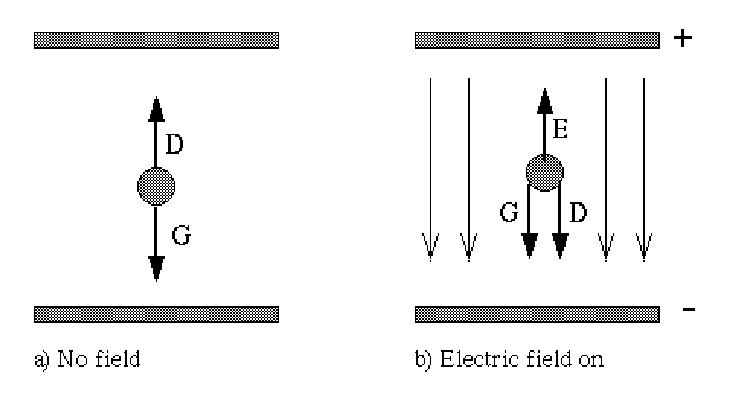
\epsfig{file=Introduction/oil_droplet.eps, height=5cm}
  \caption{
    Forces on an oil-droplet in: \newline
    \hspace*{1.5cm}
           a) Free fall          \newline
    \hspace*{1.5cm}
	   b) Electric field     \newline
    (G=Gravitation, D=Drag, E=Electric force)
  }
  \label{oil_droplet}
\end{center}
\end{figure}

His results were systematically low by about 4\% due to inaccurate
knowledge of the coefficient of viscosity. \newline
The electron charge is -e,
where $e = 1.602 \cdot 10^{-19}C$. All free particles are observed to
have values of electric charge equal to an integer times the
fundamental charge e:

\begin{equation*}
  q=n e
\end{equation*}

where the integer $n=\dots,-1,0,1,\dots$ is the electric charge
\emph{quantum number}.

\subsection*{The Nucleus}

In 1912, Ernest Rutherford and his associates discovered that the
positive charge of the atom is concentrated in a \emph{nucleus}. The
charge of the $\alpha$ particle, discovered by Becquerel, was
determined to be $2e$, and the mass of the $\alpha$ particle was
determined to be about four times the mass of the hydrogen
atom. \newline
A new particle with zero electric charge was discovered by bombarding
beryllium atoms with $\alpha$ particles. James Chadwick showed that
the new particle, the \emph{neutron}, had mass nearly equal to that of
the \emph{proton}.

\subsection*{The Bohr Model of the Atom}

In 1913, Niels Bohr made the first qunatitatively successful model of
the atom. Inspired by the work of Rutherford, Bohr made a planetary
model of the atom; with electrons moving in circular orbits about the
nucleus. This model may seem quite simple in retrospect, but for the
time it was a great advancement of science. In addition to the
classical circular orbits, the second part of Bohr's atomic model
contains a bold hypothesis of new physics. The new physics recognizes
that \emph{angular momentum} is \emph{quantized}; it can take only
certain values:

\begin{equation*}
  L = mvr = n \hbar
\end{equation*}

where $n$ is a positive integer. Solving the energy equations result
in orbits of radius:

\begin{equation*}
  r_n = \frac{n^2\hbar^2}{mke^2}
\end{equation*}

where the \emph{Bohr radius}

\begin{equation*}
  a_0 \equiv r_1 = \frac{\hbar^2}{mke^2} \approx 0.053 nm
\end{equation*}

is in the correct order of magnitude for the size of the atom!

{\bf Planc }



\chapter{Electronic Systems}
\label{ch:electronic_systems}
This chapter will be devoted to the theoretical treatment of some of the systems our program will be able to handle. The aim is to present single-particle wave functions which are good starting points 
for our many-body studies. Examples of such widely used 
single-particle wave functions are the the solutions 
to the harmonic oscillator problem or the solutions to hydrogen-like problems.

These single-particle wave functions are in turn used in constructing the so-called Slater determinant,
which together with a correlation part, is a key part of our ansatz for the trial wave functions
used in the Monte Carlo algorithm. 
\section{The Harmonic Oscillator}
The harmonic oscillator describes systems where the force 
on a particle is proportional to the distance from an equilibrium position. 
The most famous example is of course that of a mass coupled to a spring which abides to Hooke's law. However, many other systems such as molecules, motions of an atom in a lattice and phonons can be described as either one or a collection of harmonic oscillators. In this section we will first review the one particle system in one dimension and then generalize to $d$ dimensions. 
Since we confine ourselves to electronic systems, our particles are electrons. However, our formalism
can easily be extended to other particle species, such as neutrons and protons.

%Finally we will discuss the problems of interacting particles for which an analytical solution only exist in the two-particle case for specific values of $\omega$.
\subsection{One Dimension}
 The one-particle harmonic oscillator Hamiltonian in one dimension is 
%
\bea
H &=& \frac{1}{2m_e} {p}^2 + \frac 1 2 m_e\omegasq x^2,\\
     &=& - \frac{\hbar^2}{2m_e}\dd x + \frac 1 2 m_e\omegasq x^2,
\eea
%
where $\omega$ is the oscillator frequency and $m_e$ is the electron mass.  The time independent Schr\"odinger equation $H \phi = E\phi$ becomes
%
\be
- \frac{\hbar^2}{2m_e}\ddf \phi x + \frac 1 2 m_e\omegasq x^2 \phi = E\phi.
\ee
%
Before we solve this it is convenient to introduce  dimensionless variables
%
\bea
\underline x &=& \frac{x}{\sqrt{\hbar/m_e\omega}},\\
\eps &=& \frac{2E}{\hbar \omega}.
\eea
% 
Dropping the underline in $\underline x$ and using the prime notation to indicate derivation we get
%
\be
\phi''  + (\eps-x^2)\phi = 0. 
\label{eq:schrodinger}
\ee
%
This is a second-order linear homogeneous differential equation. 
To solve it we first look at the behaviour when $x\rightarrow \infty$. In this case we can neglect the $\eps$ term and get
%
\be
\phi'' = x^2\phi, \quad x\rightarrow \infty.
\label{eq:schrodingeratinf}
\ee
%
We need a function that when derivated gives back the original function times $x$. The two functions $\phi(x) = e^{\pm \frac {x^2}{2}}$ do exactly this.  Inserting them into eq.~(\ref{eq:schrodingeratinf})
%
\be
\phi'' = (x^2+1)\phi \approx x^2\phi, \quad x\rightarrow \infty.
\ee
%
Since a wave function must be normalizable, only the function $\phi(x) = e^{-\frac {x^2}{2}}$ belongs to the physical Hilbert space. The solution is therefore of the type $\phi(x) = f(x)e^{-\frac {x^2}{2}}$ for some unknown function $f$. Inserting this into eq.~(\ref{eq:schrodinger}) we end up with 
%
\be
f''-2xf'+(\eps-1)f=0.
\label{eq:power}
\ee
%
This type of equation is solved by the power series method where we assume that $f(x)$ is represented
by a polynomial in $x$, namely 
$f(x) = \Sum_{k=0}^\infty a_k x^k$. The derivatives are
%
\bea
f'  &=& \Sum_{k=0}^\infty k a_k x^{k-1},\\
f'' &=& \Sum_{k=0}^\infty k(k-1) a_k x^{k-2},
\eea
%
which inserted into eq.~(\ref{eq:power}) give
%
\be
\Sum_{k=0}^\infty  k(k-1) a_k x^{k-2} + 2k a_k x^{k} + (\eps-1)a_k x^k = 0.
\ee
%
To obtain a recursion relation we notice that the two first terms in $f''$ will be zero because of the $k(k-1)$ factor. Changing variables $k$ with $k+2$ we get
%
\be
f'' = \Sum_{k=0}^\infty k(k-1) a_k x^{k-2} = \Sum_{k=0}^\infty (k+2)(k+1) a_{k+2} x^{k}, 
\ee
%
which results in
%
\be
\Sum_{k=0}^\infty  \left[ (k+2)(k+1) a_{k+2} -(2k + 1 -\eps)a_k\right] x^k = 0,
\ee
%
which is only fulfilled for all $x$ when the terms inside the brackets vanish for all $k$, viz.,
%
\be
a_{k+2} = \frac{2k + 1 -\eps}{(k+2)(k+1)}a_k, \quad k=0,1,2,\ldots
\ee
%
and the first two coefficients, $a_0$ and $a_1$, can be chosen freely. The series will diverge for large $x$ if there are no restrictions on $\eps$. We show this by noting that for large $x$, the coefficients for large $k$ will be dominate the series
%
\be
\frac{a_{k+2}}{a_k} \simeq \frac 2 k.
\ee
%
Comparing this result with the recursion relation for the power series expansion of $e^{x^2}$
%
\bea
e^{x^2} &=& \Sum_{k=0,2,4,\ldots} b_k x^k,\\
b_k &=& \frac{1}{(\frac 1 2 k)!}
\eea
%
which gives the coefficient ratio
%
\be
\frac{b_{k+2}}{b_k} = \frac{(\frac 1 2 k)!}{(\frac 1 2 (k+2))!}=\frac 1 {\frac 1 2 k +1} \simeq \frac 2 k,
\ee
%
we see that the divergence is a fact. The only way to avoid this is by terminating the series so that $f(x)$ becomes a  polynomial with a finite number of powers in $x$. 
This is possible by restricting
%
\be
\eps = \eps_n = 2n + 1, \quad n=0,1,2,\ldots,
\label{eq:quantized_energy}
\ee
%
and choosing $a_1=0$ for even $n$ or $a_0=0$ for odd $n$. We have in other words just showed that the energy for the harmonic oscillator is quantized. To find the polynomials $f_n(x)$ we insert eq.~(\ref{eq:quantized_energy}) into eq.~(\ref{eq:power}) and get
%
\be
f_n'' - 2xf_n' + 2nf_n, \quad n=0,1,2,\ldots
\ee
%
It can be shown that the solution to these equations are the Hermite polynomials $H_n(x)$ which are defined as
%
\be
H_n(x) = e^{x^2}\left( -\sd x \right)^n e^{-x^2}.
\ee
%
Using recursion relations
\bea
H_{n+1} &=& 2xH_n -2nH_{n-1},\\
H_n' &=& 2nH_{n-1}.
\eea
the first five terms are 
\bea
H_0 &=& 1, \\
H_1 &=& 2x, \\
H_2 &=& 4x^2 -2, \\
H_3 &=& 8x^3 - 12x, \\
H_4 &=& 16x^4 - 48x^2 +12.
\eea
The Hermite polynomials have alsotwo other important properties
%
\bea
\int_{-\infty}^{\infty} H_n(x)H_m(x) e^{-x^2} &=& 0, \quad n \neq m\\
\int_{-\infty}^{\infty} H_n^2(x) e^{-x^2} &=& 2^n n! \int_{-\infty}^{\infty} e^{-x^2} = \sqrt \pi \,2^n n!, 
\eea
%
which tells us that the wave functions are orthogonal and normalized. 
Switching back to normal coordinates (that it is inserting the correct dimensions) we get 
%
\bea
\phi_n(x) &=& \left( \frac{m_e\omega}{\pi\hbar} \right)^{\frac 1 4} \frac{1}{\sqrt{2^n n!}}e^{-m_e\omega x^2/2\hbar} \, 
H_n(x\sqrt{m_e\omega /\hbar})\\
E_n &=& (n+\frac 1 2)\hbar \omega
\eea
%
We see that the ground state has a non zero energy whereas the classical counterpart has not. %which has implications
\subsection{Harmonic oscillator in $d$ dimensions}
It is fortunately very easy to solve the general $d$ dimensional case once the one dimensional case is obtained. The Hamiltonian is
%
\be
H = \Sum_{r=1}^d H_r = \Sum_{r=1}^d \left(-\frac{\hbar^2}{2m_e}\dd{x_r} + \frac 1 2 m \omegasq_r x_r^2\right), 
\ee
%
which is a sum over $d$ independent parts. This suggests a wave function on the form
%
\be
\phi_N(x_1,\ldots,x_d) = \Prod_{r=1}^d \phi_{n_r}(x_r), \quad N=n_1,\ldots,n_d.
\ee
%
If we identify $n_1=n_x$, $n_2=n_y$, $x_1=x$, $x_2=y$ and so forth, the Schr\"odinger equation 
can be written as 
\be
\phi_N^{-1}H\phi_N=E_N,
\ee
resulting in
%
\be
\Sum_{r=1}^d \left( -\frac{\hbar^2}{2m_e} \frac{\phi_{n_r}''}{\phi_{n_r}} + \frac 1 2 m \omegasq_r x_r^2 \right) = E_N.
\ee
%
This can only be fulfilled if each term in the sum is a constant that adds up to $E_N$
%
\bea
-\frac{\hbar^2}{2m_e} \frac{\phi_{n_r}''}{\phi_{n_r}} + \frac 1 2 m \omegasq_r x_r^2 &=& E_r, \quad r=1,2,\ldots,d\\
\Sum_{r=1}^d E_r &=& E_N.
\eea
%
We thus end up with $d$ one dimensional equations that we already know the solution to 
%
\bea
\phi_N(x_1,\ldots,x_d) &=& \Prod_{r=1}^d 
\left( \frac{m_e\omega_r}{\pi\hbar} \right)^{\frac 1 4} \frac{1}{\sqrt{2^{n_r} 
n_r!}}e^{-m_e\omega_r x_r^2/2\hbar}\nonumber\\ && \times H_{n_r}(x_r\sqrt{m_e\omega_r /\hbar})\\
E_N &=& \Sum_{r=1}^d (n_r+\frac 1 2)\hbar \omega_r.
\eea
%
In the special case of an isotropic oscillator potential $\omega_r=\omega$ the energy is 
%
\bea
E_N &=&  (N +\frac d 2)\hbar \omega\\
N &=& \Sum_{r=1}^d n_r. 
\eea
%
Thus all the excited states are degenerate because different combinations of $n_r$ will yield the same $N$. To calculate the spatial degeneracy $g_r(N)$ we note that $n_x = 0,1,\ldots,N$ which are $N+1$ different values. In the two dimensional case $n_y=N-n_x$ so the degeneracy is just $g_2(N)=N+1$. If we include the spin degrees of freedom, the total degeneracy $G_2(N)$ becomes
%
\be
G_2(N)=2(N+1).
\ee
%
As we add more and more electrons to the system (obeying the Pauli principle), 
they will be in the state which gives the lowest total energy for the system. If we measure how much energy is required to add or remove an electron it will depend on how many electrons $N_e$ currently 
are in the system. The energy needed will have spikes at certain magic numbers $N_e = S_r(N)$ which corresponds to the case when all degenerate statesup to a given single-particle level 
are occupied. This is given by the formula
\be
S_r(N) = \Sum_{i=1}^N G_r(i).
\ee
The resulting shell structure for the two dimensional case is displayed in table~(\ref{table:2DHOShellStructure})
\begin{table}[h!]
  \centering
  \[
  \begin{array}{r|r|r|r|r}
    N&n_x&n_y&G_2(N)&S_2(N)\\
    \hline
    0&0&0&2&2\\
    1&1/0&0/1&4&6\\
    2&2/1/0&0/1/2&6&12\\
    3&3/2/1/0&0/1/2/3&8&20\\
  \end{array}
\]
\caption{Shell structure for two dimensional harmonic oscillator including combinations of $n_x$ and $n_y$}
\label{table:2DHOShellStructure}
\end{table}
The spatial degeneracy in three dimensions case is found by noting that $n_y = 0,1,\ldots,N-n_x$ which are $N-n_x+1$ different values for each $n_x$. To get the total number of different values we have to sum over all $n_x$
%
\bea
g_3(N) &=& \Sum_{n_x=0}^N (N+1-n_x),\\
       &=& (N+1)^2 - \frac{N(N+1)}{2},\\
       &=& (N+1)(N+1-\frac N 2),\\
       &=& \frac 1 2 (N+1)(N+2),
\eea
%
which gives a total degeneracy
\be
G_3(N)= (N+1)(N+2).
\ee
The shell structure is showed in table~\ref{table:3DHOShellStructure}
\begin{table}[h!]
  \centering
  \[
  \begin{array}{r|r|r}
    N&G_3(N)&S_3(N)\\
    \hline
    0&2&2\\
    1&6&8\\
    2&10&20\\
    3&20&40\\
  \end{array}
\]
\caption{Shell structure for three dimensional harmonic oscillator}
  \label{table:3DHOShellStructure}
\end{table}
The spatial degeneracy is related to the symmetry in the potential 
%
\be
V(x_1,\ldots,x_d) = \Sum_{r=1}^d \frac 1 2 m_e\omega x_r^2 = \frac 1 2 m_e\omega r^2 = V(r),
\ee
%
because when the harmonic oscillator is isotropic, each dimension contributes the same amount of energy.

\section{Quantum Dots}
Quantum dots are a man made system of trapped electrons that share some properties with atoms, 
hence the popular name ``designer atoms''. Their size ranges between 100 nm to 1 $\mu$m which 
is much larger than a regular atom. Atoms have typically spatial extensions that are of the size of 
0.05-0.4 nm. The quantum dot is created in a semiconductor, typically gallium arsenide (GaAs), 
and confined either by a physical barier, such as an insulator like aluminum gallium arsenide (AlGaAs), 
or an electric field. The confinement gives rise to a bowl shaped potential that can be 
approximated by the harmonic oscillator potential. 
One application of the quantum dot is as the qubit in a quantum computer by manipulating the electron states. Another is in biology for fluorescent labelling of both normal and cancer cells .  
\newline

We will first consider the two dimensional quantum dot and then extend our system 
to three dimensions. The purpose is to show that as long as the two-particle repulsive Coullomb interaction does not depend on spin, that the magnetic field will only result in an 
effective harmonic oscillator potential and a constant shift in the energy spectrum. 

\subsection{Two dimensions}
We first consider the case with no electron-electron repulsion.
This means that the Hamiltonian contains only onebody operators.
The Hamiltonian is derived in \ref{app:qdhamiltonian} and the result is 
%
\bea
\hat H &=& \frac{1}{2\meff} \left(\f p - \frac e c \f A\right)^2 + \frac 1 2 \meff\omegazsq (x^2+y^2) + e\phi - \f \mu_S \cdot \f B,   
\eea
%
where $\f A$ and $\phi$ is the vector and scalar potentials associated with the external electromagnetic field. The last term in the Hamiltonian is the coupling of the electron spin magnetic moment $\f \mu_S$, to the magnetic field and $\meff$ is the effective electron mass. We will consider the special case of a constant and uniform magnetic field along the z-axis, $\f B=(0,0,B)$, and no electric field. The vector and scalar potentials are related to the electromagnetic field by the equations
%
\bea
\f E &=& -\frac 1 c \pdf {\f A} t - \nabla \phi\\
\f B &=& \nabla \times A. 
\eea
%
It is easy to see that we can only obtain a constant magnetic field if also $\f A$ is constant in time. The scalar potential is now given by
%
\be
\nabla \phi = 0,
\ee
%
which has  only the solution $\phi = k$ where $k$ is a constant. We will however set $k=0$ for the rest of this derivation. Before choosing $\f A$, we expand the first term in the Hamiltonian
\be
(\f p - \frac e c \f A)^2 = p^2 - \frac e c (\f p \cdot \f A + \f A \cdot \f p) + \frac {e^2}{c^2}A^2,
\label{eq:pminusAsq} 
\ee
and in general 
\be
\f A(x,y,z) = (A_x(x,y,z), A_y(x,y,z), A_z(x,y,z) ).
\ee
This means that $\f A$ and $\f p$ will not commute unless we demand 
\be
\f A(x,y,z) = (A_x(y,z), A_y(x,z), A_z(x,y) ).
\ee
In this case we have $\nabla \cdot A = 0$, which means that we are working in the coulomb gauge. One 
possibility for the vector potential is $\f A = \frac B 2 (-y, x, 0)$ and by inserting this into eq.~(\ref{eq:pminusAsq} ) we get
\be
(\f p - \frac e c \f A)^2 = p^2 - \frac{eB}c (xp_y - yp_x) + \frac{e^2B^2}{4c^2}(x^2 + y^2)
\ee
We note that $xp_y - yp_x = L_z$, where $L_z$ is the angular momentum operator in the z direction. Inserting this into the Hamiltonian we get
\bea
H &=&  \frac 1 {2\meff} \left[p^2 - \frac{eB}{c} L_z + \frac{e^2B^2}{4c^2}(x^2 + y^2) \right] + \nonumber \\
&&     \frac 1 2 \meff\omegazsq (x^2+y^2)  + \frac{e g_s^* B}{2\meff c} S_z
\eea
where $g_s^*$ is the effective spin-gyromagnetic factor. It is easy to check that both $L_z$ and $S_z$ commute with the Hamiltonian. This means that the solution of the 
stationary Schr\"odinger equation will be an eigenfunction of $L_z$ and $S_z$. The $L_z$ operator has a simple representation in polar coordinates 
\be
L_z = -i\hbar \left(x \pd y - y \pd x \right) = -i\hbar \pd \varphi
\ee
with eigenfunction $e^{im\varphi}$ and eigenvalue $\hbar m$. Because the angles $\varphi$ and $\varphi + 2\pi$ are required to give the same eigenfunction, $m$ is restricted to the values $m=0,\pm 1, \pm 2,\ldots$. The spin operator $S_z$ is represented by the matrix
\be
S_z = \frac \hbar 2 \begin{pmatrix} 1&0\\0&-1 \end{pmatrix}
\ee
 and its eigenfunction is the two component spinor
\be
 \f \chi = \begin{pmatrix} c_1\\c_2 \end{pmatrix}
\ee
where $|c_1|^2$ and $|c_2|^2$ are the probabilities for a state with spin up and spin down, 
respectively. The eigenvalues are $\pm \hbar/ 2$ and tell us that the spin up state has a higher energy than the spin down state. This is the Pauli equation modified with the addition of a harmonic oscillator potential and we know that the spatial part of the wave function is equal for both spinor components. More formally we write the total wave function as
\be
\f \phi = \phi \f \chi,
\ee
and split the Hamiltonian in a spatial part and a spin part
\be
H = H_\Omega + H_s, 
\ee
where
\be
H_s = \frac{e g_s^* B}{2\meff c} S_z.
\ee
The stationary Schr\"odinger equation becomes
\be
\f \chi H_\Omega \phi + \phi H_s \f \chi = E \phi \f \chi 
\ee
which separates into the following system of coupled equations
\bea
\label{eq:spatial}
 H_\Omega \phi &=& E_\Omega \phi,\\
 H_s \f \chi &=& E_s \f \chi,
\eea
where $E_\Omega + E_s = E$. Solving the last one is very easy since $H_s$ is just a constant times $S_z$
\be
E_s = \frac{e \hbar g_s^* B}{2\meff c}s, 
\ee
where $s=1/2$ for spin up and $s=-1/2$ for spin down. 
\newline
\newline
We now move on to solving eq.~(\ref{eq:spatial}). Due to the spatial symmetry in the Hamiltonian we switch to polar coordinates and define
\bea
\omega_B &=& \frac{eB}{2\meff c}\\
\omegasq &=& \omegazsq + \omega_B^2.
\eea
The spatial part of the Hamiltonian is now
\be
H_\Omega = H_{r\varphi} = -\frac{\hbar^2}{2\meff}\left(\pdd r + \frac 1 r \pd r + \frac 1  {r^2} \pdd \varphi \right) 
               + i\hbar\omega_B \pd \varphi  + \frac 1 2 \meff \omegasq r^2,
\ee
which is separable in $r$ and $\varphi$. This means that the spatial part of the wave function is also separable
\be
\phi_m(r,\varphi) =R(r)e^{im\varphi}.
\ee
Feeding this into the stationary Schr\"odinger equation results in the following linear ODE in $R(r)$
\be
 - \frac{\hbar^2}{2\meff}\left(\pdd r + \frac 1 r \pd r - \frac{m^2}{r^2} \right)R(r)
 + \frac 1 2 \meff \omegasq r^2 R(r) = \eps_m R(r),
\ee
where $\eps_m = E_\Omega-\hbar m \omega_B$. This equation is solved by using the same technique as for the one-dimensional harmonic oscillator. We omit therefore the derivation. The normalized solution is
\bea
\label{eq:radial2d}
R_{nm}(r) &=& \sqrt{\frac{2n!}{(n+|m|)!}} \beta^{(|m|+1)/2} r^{|m|}e^{-\beta r^2/2} L_n^{|m|}(\beta r^2),\\
E_\Omega = E_{nm}    &=& (2n + |m| + 1)\hbar\omega + \hbar m\omega_B ,
\eea
where $n=0,1,2,\ldots,$ and
\be
\beta = \frac{\meff \omega} \hbar,
\ee
and $L_n^{|m|}(\beta r^2)$ is the associated Laguerre polynomial which in the Rodriguez representation is defined as
\be
L_n^{m}(r) = \frac 1 {n!} e^r r^{-m} \pdn r \left(e^{-r} r^{n + m} \right). 
\ee
The first three polynomials are
\bea
L_0^{m}(r) &=& 1,\\
L_1^{m}(r) &=& -r + m + 1,\\
L_2^{m}(r) &=& \frac 1 2 r^2 -(m+2)r + \frac 1 2 (m+2)(m+1). 
\eea
In order to get $\phi_{nm}(r,\varphi)$ we just have to multiply eq.~(\ref{eq:radial2d}) with the normalized angular part. The result is
\be
\phi_{nm}(r,\varphi) = \sqrt{\frac{n!}{\pi(n+|m|)!}} \beta^{(|m|+1)/2} r^{|m|}e^{-\beta r^2/2} 
                       L_n^{|m|}(\beta r^2) e^{im\varphi}. 
\ee
The total energy of the system is
\be
E = E_{nms} = E_{nm} + E_s = (2n + |m| + 1)\hbar\omega + m\hbar\omega_B  + g_s\hbar\omega_B s,
\ee
and to analyze the effect of the magnetic field we compare this energy to 
\be
E_{B=0} = E_{nm} =(2n + |m| + 1)\hbar\omega_0.  
\ee
In this case we regain the energy spectrum of a two-dimensional harmonic oscillator 
as we should, but with different quantum numbers reflecting the change to polar coordinates. 
Clearly $N=2n+|m|$, and the shell structure is shown in table~(\ref{table:2DHO}). We see that the presence of the magnetic field makes the energy depend on the sign of $m$ and $s$. The previous degenerate states will now separate more and more as the magnetic field increases. When there are no degeneracies left, the concept of shell structure may at first seem problematic. However for small magnetic fields the ionization energy will still have peaks at the same magic numbers as for the degenerate case. Of course, for strong magnetic fields this picture breaks down. We should also mention that for some special magnetic field strengths some of the non degenerate energy levels will overlap and we can have so called accidental degeneracies. One example is when $\omega_0/\omega_B = \sqrt{(1+g_s^*)^2 - 1}$ which would make $E_{00\frac 1 2}=E_{0 -1 -\frac 1 2}$. 
\begin{table}[h!b]
  \centering
      \begin{tabular}[]{r|r|r}
      $N$&$n$&$m$\\
      \hline
      0&0&0\\
      1&0&$\pm 1$\\
      2&$0/2$&$\pm 2/0$\\
      3&$0/1$&$\pm 3/\pm 1$\\
    \end{tabular}
    \caption{Shell structure for two dimensional harmonic oscillator with polar coordinate quantum numbers}
    \label{table:2DHO}
\end{table}
%
\newline
\newline
We want to briefly mention the relationship between the wave functions of the harmonic oscillator in polar and Cartesian coordinates by comparing the wavefunctions for $N=1$. I will use atomic units and omit
 the normalization factors in order to simplify the relations. In Cartesian coordinates the wave functions  are given by
\bea
\phi_{10} &=& xe^{\frac \omega 2 (x^2+y^2)},\\
\phi_{01} &=& ye^{\frac \omega 2 (x^2+y^2)},
\eea
while in polar coordinates they are
\bea
\phi_{01} &=& re^{\frac \omega 2 r^2}e^{(i\varphi)},\\
\phi_{0 -1} &=& re^{\frac \omega 2 r^2}e^{(-i\varphi)}.
\eea
By using the following relations
\bea
e^{(\pm i\varphi)} &=& \cos \varphi \pm i\sin\varphi\\
x &=& r\cos\varphi\\
y &=& r\sin\varphi
\eea
we can write the last two wavefunctions as
\be
\phi_{0\pm1} = e^{\frac \omega 2 (x^2+y^2)} \left(x\pm iy\right).
\ee
They are thus related to each other by the normalized linear combination
\be
\phi_{0\pm1} = \frac 1 {\sqrt2} \left(\phi_{10} \pm i\phi_{01}\right).
\ee
It also tells us that the two eigenfunctions of $L_z$ are $x\pm i y$, with 
eigenvalues $\pm \hbar$. %To our knowledge there is no general formula for the transformation of the wavefunctions in different coordinate systems. 
 %The Hermite polynomial relates to the Laguerre polynomial by the equations
%\bea
%H_{2n}(x) &=& (-4)^n n! L_n^{ -\frac 1 2}(x^2),\\
%H_{2n+1}(x) &=& 2(-4)^n n! x L_n^{\frac 1 2}(x^2).
%\eea

\subsection{Three dimensions}
The only change in the Hamiltonian is the inclusion of the $z$-direction. Thus the spatial Hamiltonian reads
\be
H_\Omega =  \frac 1 {2\meff} \left[p^2 - \frac{eB}{c} L_z + \frac{e^2B^2}{4c^2}\left(x^2 + y^2\right) \right] +
    \frac 1 2 \meff\omegazsq \left(x^2+y^2\right) + \frac 1 2 \meff\omega_z^2 z^2
\ee
where $p^2$ now includes $p_z^2$. The $L_z$ operator commutes with $H_\Omega$, however, an analytical solution is only attainable when $\omega_z = \omega$ since the magnetic field 
only shifts the part of the oscillator potential that is perpendicular to the magnetic field. 
Using this and changing to polar coordinates we get
\bea
H_{r\theta\varphi} &=&  -\frac{\hbar^2}{2\meff}\left[\pdd r + \frac 2 r \pd r + \frac 1  {r^2}
\left( \frac 1 {\sin^2\theta} \pdd \varphi + \cot\theta\pd \theta + \pdd \theta\right) \right]\nonumber\\
&&               + i\hbar\omega_B \pd \varphi  + \frac 1 2 \meff \omegasq r^2.
\eea
The part inside the parenthesis is equal to the operator $-\frac{1}{\hbar^2}L^2$ which also commutes with $H_{r\theta\varphi}$. Its eigenfunctions are the spherical harmonics $Y_{lm}$ which in normalized form are
\be
\label{eq:SphericalHarmonics}
Y_{lm}(\theta,\varphi) = \delta_m\left[\frac{(2l+1)(l-|m|)!}{4\pi(l+|m|)!} \right]^{\frac 1 2}
P_l^{|m|}(\cos\theta) e^{im\varphi},
\ee
with the requirement $l=0,1,2,\ldots,$ and $m=0,\pm 1, \pm 2, \ldots,\pm l$ and where
\be
\delta_m = \begin{cases}
(-1)^m& m \geq 0,\\
1&      m \leq 0.
\end{cases}
\ee
The associated Legendre polynomials $P_l^m$ are in the Rodriguez representation defined as
\be
P_l^m(x) = \frac{(-1)^m}{2^l l!}(1-x^2)^{\frac m 2}\left( \sd x \right)^{l+m}(x^2-1)^l,\quad |m| \leq l,
\ee
and the six lowest-order associated Legendre polynomials 
are shown in table~(\ref{table:LegendrePolynomials}). The eigenvalues of $L^2$ are $\hbar^2 l(l+1)$. 
\begin{table}[h!b]
  \centering
    \begin{tabular}{r|r|r}
      $|m|$&$l$&$P_l^m(x)$\\
      \hline
      0&0&1\\
      0&1&$x$\\
      0&2&$\frac 1 2(3x^2 - 1$\\
      1&1&1$-\sqrt{1-x^2}$\\
      1&2&$-3x\sqrt{1-x^2}$\\
      2&2&$3(1-x^2)$\\
    \end{tabular}
    \caption{Lowest order associated Legendre polynomials}
    \label{table:LegendrePolynomials}
\end{table}
%
The Hamiltonian is once again separable. An ansatz for the wave function is then
\be
\phi_{lm}(r,\theta,\varphi) = R(r)Y_{lm}(\theta,\varphi). 
\ee
Inserting this into the stationary Schr\"odinger equation we end up with the differential equation
\be
- \frac{\hbar^2}{2\meff}\left(\pdd r + \frac 2 r \pd r - \frac{l(l+1)}{r^2} \right)R(r)
 + \frac 1 2 \meff \omegasq r^2 R(r) = \eps_m R(r),
\ee
which is quite similar to the two-dimensional one. The solution is
\bea
R_{nl}(r) &=& \left[\frac{2n!}{(n+l+1/2)!}\right]^{1/2} \beta^{(l+3/2)} r^l e^{-\beta r^2/2} L_n^{l+1/2}(\beta r^2),\\
E_\Omega = E_{nlm} &=& (2n+l+\frac 3 2)\hbar\omega + \hbar m\omega_B
\eea
with n=0,1,2,\ldots. As expected, there are no degenerate energy levels 
and if we set $B=0$ we regain the energy spectrum of the harmonic oscillator by identifying $N=2n+l$. 
\subsection{Two-particle system}
We will now present how the problem of a two electron quantum dot can be solved analytically for certain values of $\omega$. These results are 
taken from the article \cite{MTautQDotAnalSol} and form an  important basis for checking our 
numerical solution method and also to gain some physical insight on the role of  
correlations. The spatial Hamiltonian in two dimensions is
\be
H_{r_\varphi} = \Sum_{i=1}^2 \left[\frac 1 {2\meff}\left(\f p_i - \frac e c \f A_i \right)^2 + \frac 1 2 \meff\omegazsq r_i^2 \right] + \frac{e^2}{4\pi\eps_0 |\f r_2 - \f r_1|}.
\ee
By introducing the center-of-mass and relative coordinates we can split the Hamiltonian in two parts, one which depends on the relative coordinates only and one which depends on the center-of-mass coordinates. 
We can the use the separation of variables technique when solving the stationary Schr\"odinger equation. The coordinate transformation is given by
\bea
\f r &=& \f r_2 - \f r_1,\\
\f R &=& \frac 1 2 (\f r_1 + \f r_2),
\eea
where $\f R$ and $\f r$ are the center-of-mass term and the relative term, respectively. The momenta will also be transformed according to
\bea
\f p &=& \frac 1 2(\f p_2 - \f p_1), \\
\f P &=&  \f p_1 + \f p_2.
\eea
When $\f B$ is a constant, Maxwell's equations implies that $\f A$ must be linear
\bea
\f A(r) &=& \f A(r_2) - \f A(r_1),\\
\f A(R) &=& \frac 1 2 ( \f A(r_1) + \f A(r_2) ).
\eea
The following relations will come in handy when transforming the Hamiltonian
\bea
p_1^2 + p_2^2 &=& \frac 1 2 (P^2 + 4p^2),\\
r_1^2 + r_2^2 &=& \frac 1 2 (4R^2 + r^2),\\
|\f r_2 - \f r_1| &=& r\\
\f p_1 \cdot \f A(r_1) + \f p_2 \cdot \f A(r_2) &=& \f p \cdot \f A(r) + \f P \cdot \f A(R)\\
A_{r_1}^2 + A_{r_2}^2 &=& \frac12 A(r)^2 + 2A(R)^2
\eea
The result is
\begin{equation}
\begin{split}
H_{r_\varphi}&= \frac1{2}\left\{\frac1{2\meff} 
\left[P^2 -4\frac ec \f P \cdot \f A(R) + 4 \frac{e^2}{c^2}A(R)^2\right] 
+  2 \meff\omegazsq R^2 \right\} \\
&\;\; + 2 \biggl\{ \frac1{2\meff}\left[p^2 - \frac ec \f p \cdot \f A(r) + \frac14 \frac{e^2}{c^2}A(r)^2\right]
+  \frac18 \meff\omegazsq r^2 \\ 
& \;\; \qquad + \frac{e^2}{8\pi\eps_0 r}\biggr\},
\end{split}
\end{equation}
and by introducing
\bea
\label{eq:omegaR}
\omega_R &=& 2\omega_0\\
\omega_r &=& \frac12 \omega_0\\
\label{eq:AR}
\f A_{R} &=& 2 \f A(R)\\
\label{eq:Ar}
\f A_{r} &=& \frac12 \f A(r)
\eea
we get
\bea
H_{r_\varphi} &=& \frac 1 2\left\{\frac1{2\meff} \left[P-\frac ec \f A_{R}\right]^2
+  \frac12 \meff\omega_R^2 R^2 \right\} + \nonumber \\
&& \, 2 \left\{ \frac1{2\meff} \left[p - \frac ec \f A_{r}\right]^2
+  \frac12 \meff\omega_r r^2 + \frac{e^2}{8\pi\eps_0 r}\right\},\\
&\equiv&\frac12 H_R + 2H_r.
\eea
The wavefunction can the be written in  the product form  as 
\be
\Psi(\f r,\f R) = \psi_r(\f r) \psi_R(\f R)
\ee
and when inserted into the Schr\"odinger $H\Psi = E\Psi$ we end up solving the system of equations
\bea
\label{eq:rel}
H_r \psi_r &=& E_r \psi_r\\
\label{eq:com}
H_R \psi_R &=& E_R \psi_R
\eea
 with total energy
\be
E = \frac12 E_R + 2E_r.
\ee
The solution to the center-of-mass problem, eq~(\ref{eq:com}) is the same as for the one particle case. The energy will be
\be
E_R = E_{NM} = 2(N + |M| + 1)\hbar \omega + 2\hbar M \omega_{B} 
\ee
where the extra factor of two in comes from eq.~(\ref{eq:AR}) and eq.~(\ref{eq:omegaR}).
\newline

We now move on to solve eq.~(\ref{eq:rel}) which is the relative part. The presence of the $1/r$ term makes it impossible to get a general closed-form solution. 
Such solutions only exist for particular values of $\omega$ that can be 
found by solving $a_n=0$ where $a_n$ is given by the the following recurrence relation
\bea
a_0&\neq&0\\
a_1&=&\frac 1 {a_0'(2|m|+1)} \sqrt{\frac {2 \hbar} {\meff\omega}}a_0\\
a_n &=& \frac{1}{n(n+2|m|)}\biggl\{\frac 1 {a_0'}\sqrt{\frac {2\hbar} {\meff\omega}}a_{n-1}\nonumber\\ 
&&+ \left[2\left(n+|m|-1\right) -\eps_{nm}\right]a_{n-2}\biggr\}, \quad n\geq2
\eea
where 
\be
a_0' = \frac{8\pi\eps_0\hbar^2}{2\meff e^2},
\ee
and
\be
\eps_{nm} = 2(|m|+n),  \quad n\geq2. 
\ee
The energy is given by
\be
E_r =E_{nm} = \frac 1 2(|m|+n)\hbar\omega + \frac12 m \hbar\omega_B. 
\ee
The procedure is to chose a value for $n$ and insert $\eps_{nm}$ into the expression for $a_n$ and then solve $a_n=0$ with respect to $\omega$. The ground state is given by $n=2$ and $m=0$ which gives $\omega=1$ and energy $E_r=\hbar$. The ground state of the center of mass part is given by $N=M=0$ which gives energy $E_R=2\hbar$. The total energy for the ground state of a two particle quantum dot is then $E=3\hbar$. The energy for the non-interacting case is just the one particle energy multiplied with two (the spin part cancels) and will for the ground state be equal to the center of mass energy. We see that the interaction energy is $1/3$ of the total energy.
\newline

In the three dimensional case it can be shown that we only have to make the substitution $|m|=l+1/2$ in the above expressions. The energy is
\bea
E_R = E_{NLM} = 2(2N + L + \frac32)\hbar\omega + 2\hbar M \omega_{B}\\
E_r = E_{nlm} = \frac 1 2(n+l+\frac12)\hbar\omega + \frac12 m \hbar\omega_B.  
\eea
The ground state energy is given by $n=2,l=m=0$ and $N=L=M=0$ for the relative and center of mass part, respectively. This gives $\omega=1/2$ and total energy $E=2\hbar$ from which the interaction part contributes $1/4$. We see that the interaction part is more important in the two dimensional case. This is expected since lower dimensionalities give less degrees of freedom. 

\section{Atomic systems}
We want to show that our program is capable of solving multi electron atoms by using the Slater determinant of hydrogen like wavefunctions. These wavefunctions are found by solving the stationary Schr\"odinger equation for one electron in an atom with $Z$ protons. This is a $Z+1$ body problem that is in general not analytically solvable. Howewer, we can exploit that the nucleus is much heavier than the electron by many orders of magnitude. The effect will be that the nucleus is almost at rest compared to the electron. We will therefore approximate the problem by treating the nucleus as having no kinetic energy. Though one should note that this approximation will only be accurate if the momenta of the nucleus and the electron is of the same order of magnitude. This is easily shown by comparing their kinetic energy $T$ given by
\bea
T_e &=& \frac {P_e^2}{2m_e}\\
T_Z &=& \frac {P_Z^2}{2Zm_p}.
\eea
We see that only if $P_e \approx P_Z$ will $T_e >> T_p$. This is one step in the Born-Oppenheimer (BO) approximation and is very important in molecular physics. 
\subsection{Hydrogen like wave functions}
The Hamiltonian is
\be
H = -\frac{\hbar^2}{2m_e}\nabla^2 - \frac{Ze^2}{4\pi\eps_0}\frac1r, 
\ee
and is spherically symmetric. This means that, as for the three dimensional quantum dot, the wavefunction is separable and we can use the ansatz
\be
\phi_{lm}(r,\theta,\varphi) = R(r)Y_{lm}(\theta,\varphi)
\ee
where $Y_{lm}$ are the spherical harmonics defined in eq.~(\ref{eq:SphericalHarmonics}). The Schr\"odinger equation reads
\be
\left\{-\frac{\hbar^2}{2m_e}\left[\pdd r + \frac 2 r \pd r + \frac {l(l+1)}{r^2} \right]
 - \frac{Ze^2}{4\pi\eps_0}\frac{1}r \right\}R(r) = ER(r). 
\ee
The derivation of its solution is given in standard quantum mechanical textbooks, see for example \cite{book:Hemmer}. The result is 
\bea
E_{n} &=& - \frac{\hbar^2}{2 m_e a_0^2}\frac{Z^2}{n^2},\\
R_{nl}(r) &=& -\left[\frac{4(n-l-1)!}{a^3n^4[(n+l)!]^3} \right]^{\frac12}
(\rho_n r)^l e^{-\frac12 \rho_n r}L_{n+l}^{2l+1}(\rho_n r)\\
n&=&1,2,\ldots,\\
l&=&0,1,\ldots,n-1, 
\eea
where $\rho_n=2/na$ and $a=a_0/Z$. Comparing this energy with that of the three dimensional harmonic oscillator we see that it only depends on one quantum number. To calculate the spatial degeneracy we see that for each $n$, $l$ can take $n-1$ different values. We also know that for each $l$, $m$ can take $g_l=2(2l+1)$ different values and is called a subshell. By summing this we get
\be
g_n = \Sum_{l=0}^{n-1} (2l+1) = 2\frac{n(n-1)}2 +n = n^2,
\ee
and when including spin degrees of freedom the total degeneracy is $G_n = 2n^2$. The shell structure is shown in table \ref{table:ShellStructureAtom}
\begin{table}[h!]
  \centering
  \[
  \begin{array}{r|c|r|r|r|r}
    nl&m&G_l&S_l&G_n&S_n\\
    \hline
    1s&0&2&2&2&2\\
    \hline
    2s&0&2&4& &\\
    2p&-1,0,1&6&10&8&10\\
    \hline
    3s&0&2&12& & \\
    3p&-1,0,1&6&18& &\\
    3d&-2,-1,0,1,2&10&28&18&28\\
  \end{array}
\]
\caption{Shell structure in an atom using spectroscopic notation. The number of orbitals in each subshell is $G_l = 2g_l$ and the total number of obitals in all subshells is $S_l = \sum G_l$.}
\label{table:ShellStructureAtom}
\end{table} 

\section{Identical particle symmetry}
When dealing with systems of more than one particle it is natural to label them with a number. This is valid in classical physics even if the particles are identical because \footnote{Identical in the sense that all of their intrinsic properties like electric charge and spin are equal. In other words, there are no experiments that could detect any intrinsic differences between them.} we can always seperate the particles by observing their historical trajectories. However, this is not possible in the quantum mechanical case because observing the system would disturb it. The logical consequence of this is that interchanging a pair of particles in the wave function should not change any observable of the system. This is called particle symmetry and has measurable physical consequences. Let 
\be
\psiij = \psi(\f x_1, \ldots, \f x_i, \ldots, \f x_j, \ldots, \f x_N). 
\ee
Then particle symmetry is equivalent to the equation
\be
|\psiij|^2 = |\psiji|^2,
\ee
and has the general solution
\be
\psiji = e^{i\beta}\psiij,
\ee
where $\beta$ is a real number. To find $\beta$ we define a permutation operator $\Pij$
\be
\Pij \psiij = \psiji.
\ee
We need to know if it is Hermitian. First note that when it operates twice we must get the same wave function back
\be
\label{eq:Psq}
\Pij^2 = I
\ee
 which means that
\be
\label{eq:Pinv}
\Pij = \Pij^{-1}.
\ee
It has also been shown (reference?) that for any operator $O$ corresponding to some observable then
\be
O = \Pij^\dagger O \Pij.
\ee
In particular for $O=I$ we get $\Pij^\dagger\Pij = I$ which together with eq.~(\ref{eq:Pinv}) shows that the permutation operator is Hermitian, $\Pij^\dagger = \Pij$. Using this and eq.~(\ref{eq:Psq}) means that $\Pij$ commutes with any observable $O$, the Hamiltonian as well. This means that any eigenfunction $\psi_k$ of $H$ is also an eigenfunction of $\Pij$ with eigenvalue $p_{ij}$. Using eq.~(\ref{eq:Psq}) again we get
\bea
\Pij^2 \psi_k &=& p_{ij}^2 \psi_k\\
              &=& \psi_k
\eea
which means that $p_{ij}=\pm 1$. It can also be shown that the eigenvalue $p_{ij}$ is independent of which particles are being permutated thus $p_{ij}=p$. It is an empirical fact that wave functions with $p=1$ are symmetric $\psi_S$ and describes particles with whole integer spin, namely bosons. For $p=-1$ the wave function is anti-symmetric $\psi_A$ and describes particles with half integer spin which are fermions. This suggests that $\beta = 0$ describes a symmetric state while $\beta = \pi$ describes an anti-symmetric state. We can generalize this to include all possible two-particle permutations by the operator $\Pall$. This can be written as
\be
\Pall = \Prod_{i=1}^N\Prod_{j=i+1}^N \Pij
\ee   
and has the properties
\bea
\Pall \psi_S &=& + \psi_S\\
\Pall \psi_A &=& (-1)^{n_p} \psi_A
\eea
where $n_p$ is the total number of two-particle permutations done by $\Pall$. 
 
\subsection{Systems of non-interacting fermions} 
The Hamiltonian of such a system with $N$ particles is
\be
\Hop_0 = \Sum_{i=1}^N \hop_i
\ee
where $\hop_i$ is the one particle Hamiltonian. The eigenfunction is on the product state form
\be
\psi_{\mu}(\f x_1,\ldots,\f x_N) = \Prod_{i=1}^N  \phi_{\mu_i}(\f x_i)
\ee
where $\phi_{\mu_i}$ is an eigenfunction of $\hop_i$ and $\mu_i$ is a set of quantum numbers describing the one particle state. While $\psi_k$ is an eigenfunction of $\Hop_0$ it is not an eigenfunction of $\Pall$. However, we know that any linear combination of different product states is also an eigenfunction of $H$. It turns out that the following linear combination is an eigenstate of $\Pall$
\be
\psi_\mu(\f x_1,\ldots,\f x_N) = \frac{1}{\sqrt{N!}}\left| 
  \begin{array}{cccc}
    \phi_{\mu_1}(\f x_1) & \phi_{\mu_1}(\f x_2) & \dots  &\phi_{\mu_1}(\f x_N) \\ %[4pt]
    \phi_{\mu_2}(\f x_1) & \phi_{\mu_2}(\f x_2) & \dots  &\phi_{\mu_2}(\f x_N) \\ %[4pt] 
    \vdots    & \vdots    & \ddots &\vdots    \\ %[4pt]
    \phi_{\mu_N}(\f x_1) & \phi_{\mu_N}(\f x_2) & \dots  &\phi_{\mu_N}(\f x_N)
  \end{array}
\right|
\ee 
which is called the Slater determinant. If we have the case $\mu_i=\mu_j$ for some $i$ and $j$ then two of the rows will be equal and render the determinant zero. This tells us that two fermions cannot occupy the same state and is a consequence of the well-known Pauli exclusion principle. Changing two particles is equal to changing two columns and gives a sign change in the determinant.
\newline

As an example we will consider the Beryllium atom which has four electrons. The Slater determinant of the ground state configuration is
\be
\psi_{}(\f x_1,\f x_2) = \frac{1}{\sqrt{2!}}\left| 
  \begin{array}{cc}
    \phi_{00\uparrow}(\f x_1) & \phi_{00\uparrow}(\f x_2) \\
    \phi_{00\downarrow}(\f x_1) & \phi_{00\downarrow}(\f x_2) \\
  \end{array}
\right|
\ee
\subsection{Systems of interacting fermions}
\label{section:InteractingFermions}
When the particles are interacting the Hamiltonian is
\be
\Hop = \Hop_0 + \Hop_I
\ee
where $\Hop_I$ is the interaction part. While the Slater determinant is now no longer a solution to the system it still serve a purpose. If the set $\{ \phi_{\mu_i}\}$ of one particle functions form a complete basis then the set $\{\psi_{\mu}\}$ of Slater determinants can be shown to also form a complete basis. This means we can expand the eigenfunction of $\Hop$ as
\be
\Psi = \Sum_\mu c_\mu \psi_\mu
\ee
where $\mu$ is a specific configuration and $|c_\mu|^2$ is the probability of that configuration. If we then can numerically find the coefficients $c_\mu$, we have in principle solved the problem. This is the starting point of the Configuration-Interaction (CI) method described in (referanse). 
%eq.~(\ref{})
%We have choosen to scale the equation i atomic units explained in
%\begin{pmatrix} c_1\\c_2 \end{pmatrix}
%Note that $\nabla^2$ in polar coordinates contains the term
%\be
%\pdd \varphi = - \frac 1 {\hbar^2} L_z^2
%\ee
%which means that the harmonic oscillator.


\chapter{Numerical Methods}
This chapter is devoted to the treatment of some of the most common numerical methods in quantum mechanics. Any numerical method will have to use some kind of approximation to solve the problem. In quantum mechanics it is most common to approximate either the wave function or the interaction part of the Hamiltonian. 

\section{Monte Carlo}
There is no precise definition of the large range of numerical methods that falls under the Monte Carlo (MC) category. Howewer, they can be described as  statistical simulation methods in the sense that they use a sequence of random numbers in the simulation. Monte Carlo methods are used in many different fields such as chemistry, biology, physics, biology, mathematics and computational finance. 
\newline

The MC methods are especially useful when the degrees of freedom in the system are many, strongly coupled and hard to simplify. Examples are fluids, disordered materials, interacting baryons such as nucleons and strongly coupled solids. In mathematics it is used in the calculation of large dimensional integrals often with complicated boundary conditions.   

The $MC$ method is particularly suited for studying physical systems that are governed by a probability distribution function (PDF). The reason is that we can simulate the system directly and calculate any observable in case we have an analytical expression for. This is contrary to the standard deterministic approach which usually involves finding and solving a set of partial differential equations. The statistical interpretation of the quantum mechanical wavefunction makes the (MC) method well suited here as well.  

\subsection{The variatonal principle}
The expectation value of the energy is
\be
\label{eq:VarEnergy}
 \expval {\Hop} = E[\PsiTrial] = \frac {\braket \Hop {\PsiTrial}}{\norm \PsiTrial} = 
\frac{\int d{\bf X}\PsiTrial^*({\bf X})H({\bf X})\PsiTrial({\bf X})}
{\int d{\bf X}\PsiTrial^*({\bf X})\PsiTrial({\bf X})},
\ee
where $\f X$ is a shorthand for the set of position vectors $\f x_1, \ldots, \f x_N$, and $\PsiTrial$ is a trial wave function that is parameterized with the scalars $\varparam$. We now expand the trial wave function in the energy eigenbasis (the exact eigenvavectors of a given  Hamiltonian). These eigenvectors form a complete set of orthonormal eigenfunctions
\be
\PsiTrial = \Sum_i a_i\psi_i. 
\ee
Inserting this into the expression for the energy expectation value we get
\be
E[\PsiTrial]= \frac{\Sum_{ij}(a_i^*a_j\int \psi_i^*\Hop \psi_j d\f X)}
{\Sum_{ij}(a_i^*a_j\int \psi_i^* \psi_j d\f X)}.
\ee
Using that $\Hop \psi_i = E_i \psi_i$ and the orthonormality condition $\int \psi_i^* \psi_j=\delta_{ij}$ gives
\be
E[\PsiTrial]= \frac{\Sum_i |a_i|^2 E_i}{\Sum_i |a_i|^2} \geq E_0,
\ee
where $E_0$ is the energy of the ground state. 
We have therefore proved that the variational energy is an upper bound to the exact ground state energy. This important property will be used to find a good wave function. 
The use of the uniform distribution to sample the  integral for the expectation value of the energy
would lead to a highly inefficient algorithm. The sampling method must generate points where the integrand is large. To achieve this we express eq.~(\ref{eq:VarEnergy}) in terms of the PDF
\be
P(\f X) = \frac{|\PsiTrial|^2}{\int |\PsiTrial|^2}
\ee
by defining a local energy as
\be
E_L(\f X) \equiv \frac1{\PsiTrial}\Hop \PsiTrial.
\ee
The energy expectation value can now be written as a weighted average of the local energy
\be
E[\PsiTrial] = \expval {E_L}_P = \int P(\f X) E_L(\f X)d\f X 
\approx \frac 1 M \Sum_{i=1}^M P(\f X_i) E_L(\f X_i),
\ee
where $M$ is the number of MC cycles. We will use the Metropolis algorithm to sample from $P$. That is a method based on a stochastic random walk and will introduce a statistical error $\eps$ in our computations of the local energy. The error is equal to the standard deviation of the distribution of $\expval {E_L}_P$ that we get by using different samples of $P$ in each calculation of $\expval {E_L}_P$. The standard deviation is given by the square root of the variance $\sigma_{E_L}^2$ of the local energy,  defined as
\bea
\sigma_{E_L}^2 &\equiv& \expval{(E_L - \expval{E_L}_{P})^2}_{P}\\
         &=& \expval{E_L^2}_{P} - 2 \expval{E_L}_{P}^2 + \expval{E_L}_{P}^2,\\
         &=& \expval{E_L^2}_{P} -  \expval{E_L}_{P}^2.
\eea
 It is easy to check that if the trial wave function is an exact eigenfunction then the variance is zero. This property can be used to find the optimal parameters because we do not always know what the lowest energy is while the lowest variance is always zero. It is possible to show (see appendix \ref{section:StatisticalAnalysis}) that the error is given by
\be
\eps = \sqrt{\frac {\tau}{M}} \sigma_{E_L}.
\ee
where $\tau$ is the autocorrelation time. It is equal to one if there are no correlations. This means that assuming no correlations gives a too optimistic estimate of the error. The standard way of computing $\tau$ is very time consuming so we will rather use the so-called blocking method which is an approximative method that gives reliable results for the standard error and standard deviation. 
\subsection{The Metropolis algorithm}
Generating a set of points that are distributed according to some known PDF can be a rather non-trivial task. The starting point is the uniform distribution generated by a pseudo random number generator and we have to transform it into the desired PDF. One technique is the inversion method which can give us an analytic transformation function. Take $X$ as a random variate whose PDF is the uniform distribution $u(x)$. Let $Y$ be the random variate from our desired PDF $p(y)$. The objective is to find a function $f$ so that $f(x)=y$. It can be shown that
\bea
p(y) = p(f(x)) &=& u(x)\left| \frac{dx}{dy}\right|,\\
&=& u(f^{-1}(y)) \left| \frac{df^{-1}(y)}{dy}\right|.
\eea
By using that $u(x)=1$ since it is defined by the  uniform distribution, we get
\be
p(y)dy = df\inv(y).
\ee
Integrating both sides leads to 
\be
f^{-1}(y) = \Int_{-\infty}^{y} p(y')dy' = P(y),
\ee
where $P(y)$ is the cumulative probability of $p(y)$. This means that
\be
f(x) = P\inv (x). 
\ee
The problem with this method is that the integral of $p(y)$ must be known and invertible. If not we could generate it numerically but that leads normally to a more  inefficient algorithm. One important application of the inversion method is the so-called Box-Muller algorithm which generates a pair of Gaussian random numbers $(y_1,y_2)$ with variance $\sigma^2$ and mean value $\mu$, given a pair of uniformly distributed random numbers $x_1,x_2$ as input. It can be shown that (referanse?)
\bea
y_1 &=& \sigma^2 \sqrt{-2\ln{x_1}} \cos{(2\pi x_2)}  + \mu,\\
y_2 &=& \sigma^2 \sqrt{-2\ln{x_1}} \sin{(2\pi x_2)} + \mu.
\eea
which will be used in the program
\newline

The Metropolis algorithm is a way of generating a distribution by constructing a Markov chain that has the desired distribution as its equilibrium distribution (the most likely state). The 
Markov chain will be created by a random walk in state space with the property that the next step of the walk only depends on the current state and some random number. 
All information about how the current state was reached is lost. The random walker is just a mathematical object that can represent any physical quantities. In this thesis it represents the state of the electrons which are governed by their positions. In this text we will often refer to a random walker or
just walker(s) when we discuss the simulation process. The random walker(s) represents thus a collection of samples in our state space of possible events. These samples form the basis for computing various
expectation values like the variance of the energy or the energy.  
\newline

Let the set $\{S_1,\ldots,S_N\}$ be all the available states and let $S_j$ represent the state at time $i$. Let
\be
P_{kj} \equiv P(S_k \leftarrow S_j)
\ee
be the probability of going from state $S_j$ to $S_k$ in one time step, where $S_k$ represents the state at time $i+1$. In our simulations time is used here in a loose way 
to label the different simulation steps (typically the distance between each sampling).  
It has nothing to do with the physical time of the system in consideration. Normalization and positivity of the probabilities demand that
\bea
&& 0 \leq \; P_{kj} \powi \leq 1, \quad k=1, 2, \ldots, N, \quad j=1, 2, \ldots, N\\
&&\Sum_{k=1}^N P_{kj} = 1, \quad j=1, 2, \ldots, N,
\eea
Let $p_r^{(i)}$ be the probability that the system is in state $S_r$ at time $i$. The probability distribution of the walkers can be represented by the vector
\be
\f p\powi = 
\begin{bmatrix}
p_1\powi\\
p_2\powi\\
\vdots\\
p_N\powi\\
\end{bmatrix}
\ee
with the requirements
\bea
&& 0 \leq \; p_k\powi \leq 1, \quad k=1, 2, \ldots, N\\
&&\Sum_{k=1}^N p_k\powi = 1.
\eea
The evolution of $\f p$ is
\be
p_k\powii = \Sum_j P_{kj} p_j\powi,
\label{eq:pPp}
\ee
which is equal to the matrix vector equation $\f p\powii = \f P \f p\powi$. After $m$ steps the state is
\be
\f p\powm = \f P^m \f p\powz
\ee
Assume that there exist an equilibrium distribution $\f p^*$ given by
\be
\f p^* = \f P \f p^*. 
\ee
Obviously $\f p^*$ is an eigenvector of the transition matrix $\f P$ with eigenvalue $1$. We want to write this in a different way by subtracting $p_k\powi$ and $\sum_j P_{jk} p_k\powi$ from the left and right hand side (respectively) of eq.~(\ref{eq:pPp}). This is possible since 
 $\sum_j P_{jk} = 1$. The result is
\be
p_k\powii - p_k\powi = \Sum_j P_{kj} p_j\powi - \sum_j P_{jk} p_k\powi.
\ee
At equilibrium we must have $p_k\powii = p_k\powi$ which leads to
\be
\Sum_j P_{kj} p_j\powi = \sum_j P_{jk} p_k\powi.
\ee
The stronger condition
\be
P_{kj} p_j = P_{jk} p_k
\ee
is called detailed balance and tells us that the individual flow between pairs of states are equal. Consider now splitting the move from $S_j$ to $S_k$ in two steps, first the move is suggested with probability $\omega_{kj}$, then it is accepted with probabilty $A_{kj}$. The total probability for moving is the product
\be
\omega_{kj}A_{kj} = P_{kj}.
\ee
The detailed balance equation now reads
\be
\frac{A_{kj}}{A_{jk}} = \frac{\omega_{jk} p_k}{\omega_{kj} p_j}.
\ee
Many different choices of $A$ will satisfy this equation but the choice in the Metropolis algorithm is
\bea
A_{kj} &=& \mathrm{min} \left[1,  \frac{\omega_{jk} p_k}{\omega_{kj} p_j}\right]\\
A_{jk} &=& \mathrm{min} \left[1,  \frac{\omega_{kj} p_j}{\omega_{jk} p_k}\right]\\
A_{jj} &=& 1
\eea
This matrix has the advantage of being very easy to implement numerically and the probability distributions need not be normalized since the normalization factors cancel when computing the 
ratio between probabilities. The correspoding algorithm is to generate a uniform random number $r$ and compare it with
\be
v_{kj}  = \frac{\omega_{jk} p_k}{\omega_{kj} p_j}.
\ee
If $v_{kj} > r$ then the move is accepted. In this thesis the distribution $\f p$ corresponds to $|\Psi(\f X)|^2$. One example of a random walk is the algorithm
\be
\f Y = \f X + (r-0.5)l
\ee
where $l$ is a step length. It is easy to see that increasing $l$ would decrease sequential correlation, but unfortunately this also decreases the acceptance ratio because 
when $\f Y$ is large $|\Psi(\f X)|^2$ is small. A small acceptance ratio means that the particle will get stuck in the same place and the resulting energy or other expectation values 
would most likely be strongly biased. Generally an acceptance ratio between $0.3$ and $0.7$ is a good starting point but it really has to be investigated for each experiment.
\newline

The optimal solution would be to take large steps to regions were $|\Psi(\f X)|^2$ is large. It turns out that there exists a possible procedure for doing this based on the so-called 
Fokker-Planck equation. It pushes the walkers according to the gradient of the distribution. The move mimics an isotropic diffusion process with a drift force $F$. The random walk is now given by
\be
\f Y = \f X + D\f F(\f X)\delta t + \chi
\ee  
where $D$ is the diffusion constant and $\chi$ is a Gaussian random variable with mean value equal zero and variance $2D\delta t$. The force term is given by
\be
\f F = \frac 1 p \nabla p  
\ee
and with $p=|\Psi|^2$ we get
\be
\f F = \frac 2 \Psi \nabla \Psi.  
\ee
Clearly the move is biased towards large $|\Psi|^2$ and is a form of importance sampling which means sampling the states that contribute the most to the physical quantity we wish to find. It can be shown that the probability for moving from $\f X$ to $\f Y$ is
\be
\omega(\f Y, \f X) = e^{\frac{-(\f Y - \f X - D \delta t \f F(\f x))^2} {4D\delta t}}. 
\ee
The acceptance matrix is then
\be
A(\f Y, \f X) = \mathrm{min} \left[1, \frac{\omega(\f X, \f Y) |\Psi(\f Y)|^2}
                                           {\omega(\f Y, \f X) |\Psi(\f X)|^2} \right]
\ee
% \subsection{Random numbers}   
% The generation of random numbers are very important in Monte Carlo methods. One may wonder how it is possible for a deterministic machine such as a computer to generate anything random other than blue screens. The answer is that a number in itself is not random, rather it is the relationship between numbers in a set that is random. Fortunately there are algorithms that can generate set of numbers that are distributed in a seemingly random way.
% We call them Pseudo random generators (PRNG) and have to important propert

%\subsection{Importance sampling}

\subsection{Trial wave function}
The choice of wave function is very important in variational Monte Carlo 
calculations. They should include the necessary physical properties and also be computationally feasible. In most electronic systems the typical trial wave function consists of either one or a linear combination of Slater determinants multiplied with a correlation term that is only a function of the inter-electronic or inter-particle distances. We remember from \ref{section:InteractingFermions} that any wave function can be expanded in the Slater determinant basis
\be
\Psi = \Sum_\mu c_\mu \psi_\mu.
\ee
where $\mu$ runs over all electronic configurations. Obviously this expansion must be terminated somewhere. 
The fact that the computation of the Slater determinant is usually the most demanding part limits the number of terms that are practically possible to include. If we only want the ground state energy it turns out that only one term in the expansion gives remarkably good results. This term corresponds to the ground state configuration and is an exact solution to the non-interacting system. Because the term incorporates no correlations it makes the choice of correlation term all the more important. Which single particle basis to use when defining the Slater determinant must be based on the system at hand. 
\newline

One important property that the wave function should have is to fulfill 
the so called \emph{cusp} condition. We know that the local energy is finite everywhere which means that the divergence in the Coulomb energy when two charged particles come close together must be cancelled by a corresponding divergence in the kinetic energy. It leads to a discontinuity on the first derivative of the wave function, hence the name cusp. For atomic systems we have both the electron-nucleus cusp and the electron-electron cusp. In the Harmonic oscillator and quantum dot case only the electron-electron cusp is present. Because the Slater determinant $\psi_\mu$ does not depend on $\rij$ when $i$ and $j$ are electrons of opposite spin, the derivative with respect to $\rij$ must be zero and $\psi_\mu$ cannot satisfy the cusp condition. However, we know that the determinant goes to zero when two parallel spin electrons approach each other. By using $\f \rij = \f x_j - \f x_i$ we can write the determinant as $\psisd(\f x_i,\f x_j, \ldots) = \psisd(\f x_i,\f x_i + \f \rij, \ldots)$. By expanding it around $\rij = 0$ we get
\be
\psisd(\f x_i,\f x_i + \f \rij, \ldots) \approx \psisd(\f x_i,\f x_i + 0, \ldots) + 
\rij \pdf \psisd \rij \Bigg|_{\rij=0} + \ldots
\ee
The first term is zero while the derivative in the second term is in general not zero. It is a constant $\rho_{ij}$ that does not depend on $\rij$ (we evaluated the derivative at $\rij = 0$), but it does depend on $i$ and $j$. In other words, for small $\rij$ values, we can write the determinant as $\psisd = \rij \rho_{ij}$. It can be shown (see \cite{book:Hammond}) that the electronic cusp condition gives an equation of the form
\be
\frac{1}{\rho_{ij}} \pdf {\rho_{ij}} \rij \Bigg|_{\rij=0} = f(l)
\ee 
 where $f$ depends on the Schr\"odinger equation and $l=1$ applies to the case of particles with equal spin values and opposite spin values, respectively. This equation can never be fulfilled by the Slater determinant which means that the correlation part must do it. If we choose a wave function on the product form $\Psi = \psisd \psicorr$ it can be shown that the cusp condition is equal to
\be
\frac 1 \psicorr \pdf \psicorr \rij \Bigg|_{\rij=0} = 
\begin{cases} 
1 & \text{opposite spin}\\
\frac 1 3 & \text{paralell spin}
\end{cases}
\ee
for the two dimensional case and
\be
\frac 1 \psicorr \pdf \psicorr \rij \Bigg|_{\rij=0} = 
\begin{cases} 
\frac 1 2 & \text{opposite spin}\\
\frac 1 4 & \text{paralell spin}
\end{cases}
\ee
in three dimensions. One popular type of correlation function is the Pade-Jastrow form
\be
\psicorr = e^U
\ee 
where
\be
U = \Sum_{i=1}^N \Sum_{j=i+1}^N \uij
\ee
and
\be
\uij = \frac{\Sum_{k=1}^n \gamma_k \rij^k}{1 + \Sum_{k=1}^n \beta_k \rij^k}. 
\ee
In this case we have
\be
\frac 1 \psicorr \pdf \psicorr \rij \Bigg|_{\rij=0} = \gamma_1
\ee
for the cusp condition. We will use the Pade-Jastrow form in this thesis.   
 
\subsection{Optimization techniques}
The problem of finding a global minima in a multidimensional function is not easy. When we add statistical noise it becomes even harder. We will try a method introduced by A. Harju in \cite{article:Harju1997} called the Stochastic Gradient Approximation (SGA) method. It uses the statistical noise to its advantage to avoid getting stuck in a local minima. The method bears some resemblance to the Simulated Annealing technique \cite{book:NumericalRecipiesInC++}. The SGA is an iterative scheme given by the equation
\be
\f \alpha_{i+1} = \f \alpha_{i} - \ell_i \nabla_{\f \alpha} \hat O(\f \alpha)
\ee
where $\alpha$ is the parameter vector for the total wave function and $\hat O$ is some observable like the local energy or variance. The parameter $\ell_i$ is a step length that should satisfy the conditions
\be 
\Sum_{i=1} \ell_i^2 < \Sum_{i=1} \ell_i = \infty.
\ee
A simple choice is $\ell_i = 1/i$ but we will use the more complex scheme
\be
\ell_i = \ell_0 \frac{1}{j_i^{k}}
\ee
where $j_1=0$, $1/2 < k \leq 1$ and
\be
j_{i+1} = 
\begin{cases}
\frac{j_i}2 & \text{if sign$(\pdf{\hat O}{\alpha_j})_i = $ 
                       sign$(\pdf{\hat O}{\alpha_j})_{i-1}$}\\ 
j_i + 1 & \text{if sign$(\pdf{\hat O}{\alpha_j})_i \neq $ 
                       sign$(\pdf{\hat O}{\alpha_j})_{i-1}$}
\end{cases}
\ee
The idea is that if there is no sign change in the derivative of the $j$'th component of $\f \alpha$ then we have not yet reached the minimum and want to increase the step length to increase efficiency. If there has been a sign change, then we have passed the minimum and must decrease the step length. The derivative of the local energy can be shown to be \cite{article:Lin2000}
\bea
\pdf {E(\f \alpha)}{\alpha_j} &=& \pd {\alpha_j} \frac{\int \Psi \Hop \Psi}{\int \Psi^2}\\
\label{eq:EnergyGradient}
&=& 2\expval{E_L \frac{\Psi'}{\Psi}} - 2\expval{E_L}\expval{\frac{\Psi'}{\Psi}}
\eea
where
\be
\Psi' = \pdf {\Psi}{\alpha_j}.
\ee
Similar it is shown in ref.~\cite{article:Umrigar2005} that the derivative of the variance is
\bea
\pdf {\sigma^2(\f \alpha)}{\alpha_j} &=& \pd {\alpha_j} 
\frac{\int \Psi^2 (E_L -\expval{E_L})^2}{\int \Psi^2}\\
&=& 2 \biggl[\expval{E_L'(E_L - \expval{E_L})} +  \expval{E_L^2\frac{\Psi'}{\Psi}}  
-  \expval{E_L^2}\expval{\frac{\Psi'}{\Psi}}  \nonumber \\
\label{eq:VarianceGradient}
&&\quad - 2\expval{E_L}\expval{(E_L - \expval{E_L})\frac{\Psi'}{\Psi}} \biggr]
\eea
where
\be
E_L' = \pdf {E_L}{\alpha_j}.
\ee
Variance minimization is most frequently used because it is more efficient than straightforward energy minimization. This is because it is possible to lower the energy on the finite set of MC configurations while the true expectation value is actually raised \cite{article:Umrigar2005}. The problem with variance optimization is that the parameter set for the  lowest variance may not coincide with that for the lowest energy. The SGA algorithm allows for minimizing both energy and variance and use a wheighted mean of the two sets of parameters as the optimal one. The expressions for the derivative of the energy and variance involves computing the parameter gradient of the wavefunction and local energy which is hard to optimize and therefore computationally costly. This will be discussed in greater detail in the implementation chapter. The number of random walkers $N_W$ used to compute the expectation values in eq.~(\ref{eq:EnergyGradient}) and eq.~(\ref{eq:VarianceGradient}) controls the amount of noise in the SGA algorithm. 
%\section{Hartree-Fock}
%\section{Configuration Interaction}


\chapter{Implementation}

In this chapter we will outline the program structure. We will
demonstrate the flexibility as well as the limitations of our
implementation.


%%%%%%%%%%%%%%%%%%%%%%%%%%%%%%%%%%%%%%%%%%%%%%%%%%%%%%%%%%%%%%%%%%%%
%                                                                  %
%                      Structure of the QMC Program                %
%                                                                  %
%%%%%%%%%%%%%%%%%%%%%%%%%%%%%%%%%%%%%%%%%% %%%%%%%%%%%%%%%%%%%%%%%%%
\section{Structure the QMC Program}


%%%%%%%%%%%%%%%%%%%%  Programming Philosophy  %%%%%%%%%%%%%%%%%%%%%%
\subsection{Programming Philosophy}

There are three major concepts concerning the implementation of any
large program:

\begin{enumerate}
  \item{} Speed - the computational time (CPU).
  \item{} Flexibility - ability to handle many different special cases.
  \item{} Readability - how easy it is to understand the program (and
  make modifications).
\end{enumerate}

In order to include flexibility, the
program should consist of many small building blocks, that may easily
be replaced by other similar blocks. The program structure should also
be legible. Often, modifications of existing programs need to be done,
either by the programmers themselves, or by other users. This task may
be very time consuming, especially if the program is difficult to
understand. The algorithms and data structure 
need to be well documented, the building blocks\footnote{Classes
  in C++, modules in Fortan90/50 etc.} should seem like natural
choices, and the variables names should be meaningful. \newline

Futhermore, programs may run for days on powerful machines in order to
accuire the desired result. Therefore, a great deal of effort must be
put into the design and development of the program. \newline


%%%%%%%%%%%%%%%%%%%% Main Program Structure %%%%%%%%%%%%%%%%%%%%%%%
\subsection{Main Program}

Our first concern is to recognice what the program is going to do, and
to form a program stucture. We divide the program into blocks, that
each preform some specific task. Figure \ref{program_stucture} illustrates
the basic structure of our main program. 

\begin{figure}[hbtp]
\begin{center}
  \epsfig{file=Implementation/program.eps, height=8cm}
  \caption{Variational Monte-Carlo program structure}
  \label{program_stucture}
\end{center}
\end{figure}

Generally, the user must provide some input to specify what the
computer is going to calculate.  After the input is specified, the
user does not need to do anything until the program is terminated. The
output should be presented in an easy and orderly fashion; either at
the end of the program execution, or by user specifications after the
run is completed. \newline

Dependent of the user input, the program will execute one or more runs
of the VMC algorithm. The program loops different configurations and
parameter settings, in order to localize an energy (or variance)
minimum. Each setting generate the input, the \emph{initial setup},
for a VMC calulation, and for each VMC run the program genrates an
\emph{output}. Typically, this output is for user deguging. For
example, if the initial parameter input is off bounds (and the program
terminates without finding an energy minimum) the user may chech these
outputs to adjust the user specified input for another run.


%%%%%%%%%%%%%%%%%%%%%%%%% Input Structure %%%%%%%%%%%%%%%%%%%%%%%%%
\subsection{Input}

The input structure is given by figure \ref{input_stucture}.

\begin{figure}[hbtp]
\begin{center}
  \epsfig{file=Implementation/input.eps, height=5.7cm}
  \caption{Input structure}
  \label{input_stucture}
\end{center}
\end{figure}

The user must specify the atom to be studied, and what state is to be
found - e.g. the He 2$^{nd}$ excited $^1S_0$-state. The trial wavefunction
must also be specified, both the variational form of the orbital
wavefuntions and of the Jastrow-factor. These choices gives raise to a
set of parameters, and the user must provide some inital guess, and
tell wich parameters is to be varied. The user must further set some
termination criteria, TC, for example number of Monte-Carlo
cycles. Some other parameters must also be set, either by the program,
or by the user; number of dimensions, output file-name(s), etc.


%%%%%%%%%%%%%%%% Loop Parameters & Configurations %%%%%%%%%%%%%%%%%
\subsection{Loop Parameters \& Configurations}

Figure \ref{loop_parameters_config} outlines the \emph{loop parameters \&
configurations} structure.

\begin{figure}[hbtp]
\begin{center}
  \epsfig{file=Implementation/loop_parameters_config.eps, height=7cm}
  \caption{Structure of parameter and configuration loop}
  \label{loop_parameters_config}
\end{center}
\end{figure}

We want to test different trial wave-function configurations;
i.e. different sets of the orbital wave-functions, and different sets
of Jastrow-factors\footnote{In our program these variations are left
  to the user, i.e. the user may only choose one configuration for
  each run.}.  \newline

For one fixed configuration, a set of variational
parameters, $\{\alpha_i\}$, is to be optimized with respect to either
minimization of energy or variance. We may start with one initial
guess of the set of parameters, $\{\alpha_i\}$, and one TC. When the
TC are met, we may improve our initial guess of parameters, and may
also change the TC. \newline 

For example, we may start with one-hundred thousand
Monte-Carlo cyles, make a local variation of the parameters, and move
our next parameter guess to the energy minimum of that local
variation. When the movement is no longer uni-directional we can
increase the TC to one million cycles, and may also reduce the degree
of variation. In this way, one run of the program may pinpoint
the energy-minimum with quite good accuracy, without too great expense
of computational time.

%%%%%%%%%%%%%%%%%%%%%%%%%% Initial Setup %%%%%%%%%%%%%%%%%%%%%%%%%%
\subsection{Initial Setup}

To begin one VMC run, a complete initial setup must be set; figure
\ref{initial_setup}. 

\begin{figure}[hbtp]
\begin{center}
  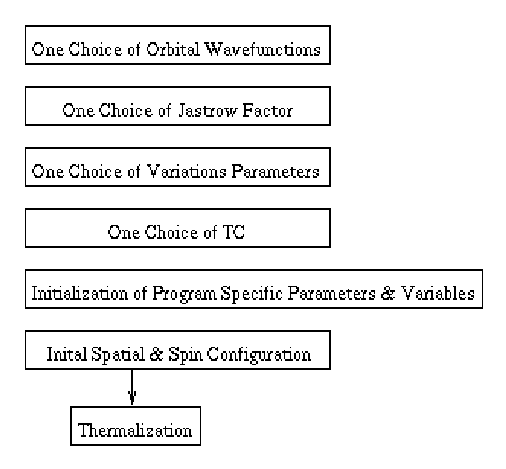
\epsfig{file=Implementation/initial_setup.eps, height=7.5cm}
  \caption{Initial setup}
  \label{initial_setup}
\end{center}
\end{figure}

In addition to the choice of trial wave-function, variational
parameters and TC, the program must initialize several parameters and
variables\footnote{These issues will be addressed {\bf
    \emph{later}}. }. Also, initial spatial coordinates of each
particle, and their respective spin, must be set.

The metropolis algorithm, {\bf \emph{described in
    section \ref{metropolis} }}, duplicates the behavior of the
wave-function. Before we begin the VMC sample, we want to make sure
that the particles initial positions are representative with respect
to the wave-function. Therefore, the metropolis algorithm is applied
several times to randomly chosen spatial and spin coordinates; the
coordinates are \emph{thermalized}.


%%%%%%%%%%%%%%%%%%%%%%%%%%%%%% VMC %%%%%%%%%%%%%%%%%%%%%%%%%%%%%%%%
\subsection{VMC}

Figure \ref{vmc} illustrates the basic principles of the different VMC
algorithms; all of which we wish to study in this thesis. 


\begin{figure}[hbtp]
\begin{center}
 % \epsfig{file=Implementation/vmc.eps, height=8.8cm}
  \input{Implementation/vmc.eepicemu}
  \caption{Three different algorithms for VMC: \newline
  (a) Move all/none particles \newline
  (b) Move one/no particle \newline
  (c) Move some particles}
  \label{vmc}
\end{center}
\end{figure}

In the first algorithm, figure \ref{vmc} (a), either all, or none, of
the particles are moved. This algorithm is easy to implement, but is
the most time-consuming of the three\footnote{Even though it is easy
  to implement, we will optimize our program with respect to the other
  two VMC algorithms. So, this ease is not reflexted in the code
  presented in \emph{?????}.}. In the second algorithm, depicted 
in figure \ref{vmc} (b), we sample the local energy after only one/no
particle is moved. In figure \ref{vmc} (c) we move some particles; 
we move one particle at a time, and conduct induvidual metropolis tests,
before we updating the local energy.

The \emph{Propose move} algorithm is depicted in figure \ref{propose_move}.

\begin{figure}[hbtp]
\begin{center}
  \epsfig{file=Implementation/propose_move.eps, height=3.8cm}
  \caption{Structure of \emph{Propose move}; proposed displacement of
    one particle}
  \label{propose_move}
\end{center}
\end{figure}

The \emph{Spin Flip} algorithm means that the particle may undergo a
spin flip with a randomly chosen particle. If the two particle have
the same spin, nothing happens. If the two particles have
different spin, the spins are exchanged. \newline
Two possible approches for the \emph{Randomize Position} algoritm:

\begin{enumerate}
  \item{}
    Variate position around the particles current location:

    \begin{equation*}
      x_{new}=x_{old}+\text{\small{RANDOM}}
    \end{equation*}

    where RANDOM is a random number based on e.g. a uniform distribution
    or a gaussian distribution.
  \item{}
    Importance Sampling:

    \begin{equation*}
      x_{new}=\Upsilon(\text{\small{RANDOM}})
    \end{equation*}

    where the function $\Upsilon$ duplicate the behaviour of the
    wave-function.
\end{enumerate}




%%%%%%%%%%%%%%%%%%%%%%%%%%%%%%%%%%%%%%%%%%%%%%%%%%%%%%%%%%%%%%%%%%%%%%
%                                                                    %
%                           Data Structure                           %
%                                                                    %
%%%%%%%%%%%%%%%%%%%%%%%%%%%%%%%%%%%%%%%%%%%%%%%%%%%%%%%%%%%%%%%%%%%%%%

\section{Data Structure}

We keep the Slater determinant and correlation wave-function in
separate classes. Let us start out with the correlation. For the
Metropolis step we need the ratio between the new and the old
wave-functions. Furthermore, we need the value of the correlation, and
its first and second derivatives, in order to preform a sample of the
local energy. \newline
We limit our attention to correlations, $G$ equal either $J$ or $e^J$,
where the Jastrow-factor is given by: 

\begin{equation}
  J = \sum_{i=0}^{\bar{N}}\sum_{j > i} f_{ij}
\end{equation}

where $N$ is the number of particles, $\bar{N}=N-1$, and

\begin{equation}
  f_{ij} = f(r_{ij})
\end{equation}

where $r_{ij}$ is the inter-electronic distance between electron $i$
and electron $j$.

Before we give the structure of the correlation, we first establish
classes to keep track of the inter-electronic distances,
\emph{Distance} and \emph{DistanceDiff}, the values of the $f_{ij}$'s,
\emph{Jastrow} and \emph{JastrowDiff}, and the derivatives,
\emph{Derivatives}.




%%%%%%%%%%%%%%%%%%%%% Distance and DistanceDiff %%%%%%%%%%%%%%%%%%%%
\subsection{Distance and DistanceDiff} 

The two classes, \emph{Distance} and \emph{DistanceDiff}, keep track
of the inter-electronic distances.  \newline
For \emph{Distance}, $r_{ij}$ is given by:

\begin{equation}
  r_{ij} = \left[
  \begin{array}{ccccccccc}
    0&r_{01}&r_{02}&\dots & r_{0i} &\dots &\dots & r_{0 \bar{N}} \\
    0&  0   &r_{12}&\dots & r_{1i} &\dots &\dots & r_{1 \bar{N}} \\
    0&  0   &  0   &\ddots& \vdots &\dots &\dots & \vdots       \\
    0&  0   &  0   &0& r_{\bar{i}i}&\dots &\dots & \vdots       \\
    0&  0   &  0   &  0   &  0&r_{ii^{^+}}&\dots & r_{i \bar{N}} \\
    0&  0   &  0   &  0   &   0    &  0   &\ddots& \vdots \\
    0&  0   &  0   &  0   &   0    &  0   & 0    &r_{\bar{\bar{N}} \bar{N}} \\
    0&  0   &  0   &  0   &   0    &  0   & 0    &  0
  \end{array} \right]
\label{r_ij}
\end{equation}

where $\bar{i}=i-1$, $i^{^+}=i+1$, $\bar{N}=N-1$ and
$\bar{\bar{N}}=N-2$. This information is stored in a single array of
length $N\dot(N-1)/2$, 

\begin{equation}
  \begin{array}{ccccc}
  rij =
  &|\underbrace{r_{01}, r_{02}, \dots, r_{0 \bar{N}} }
  &|\underbrace{ r_{12}, \dots, r_{1 \bar{N}} }
  &| \dots &|\underbrace{ r_{\bar{\bar{N}} \bar{N}} }  >\\
  & N-1 & N-2 & & 1\phantom{ii}
  \end{array}
  \label{r_ij_array}
\end{equation}

With a proposed move of electron $i$, only $N-1$ values need to be
updated. These values are stored in 

\begin{equation}
  rij\_new\_column = | r_{0i}, r_{1i}, \dots, r_{\bar{i}i}, r_{ii^{^+}},
  \dots, r_{i \bar{N}} >
\end{equation}

If the move is accepted, the values of \emph{rij\_new\_column} replace the
corresponding values in $rij$.

\emph{Distance} and
\emph{DistanceDiff} are quite similar, except \emph{DistanceDiff}
allows a variation of a coordinate.
For the \emph{DistanceDiff} class, the upper triangular matrix $r_{ij}$
is

\begin{equation}
  r_{ij} = \left[
  \begin{array}{ccccc}
    0 & r_{01}(\xi_1+h) & r_{02}(\xi_2+h)&\dots & r_{0 \bar{N}}(\xi_{\bar{N}}+h) \\
    0 &        0        & r_{12}(\xi_2+h)&\dots & r_{1 \bar{N}}(\xi_{\bar{N}}+h) \\
    0 &        0        &          0            &\ddots &  \vdots       \\
    0 &        0        &          0            &   0   &r_{\bar{\bar{N}} \bar{N}}(\xi_{\bar{N}}+h) \\
    0 &        0        &          0            &   0   &   0  
  \end{array} \right]
\label{r_ij_Diff}
\end{equation}

where $\xi$ is one of the cartesian coordinates. 

\begin{figure}[hbtp]
\begin{center}
  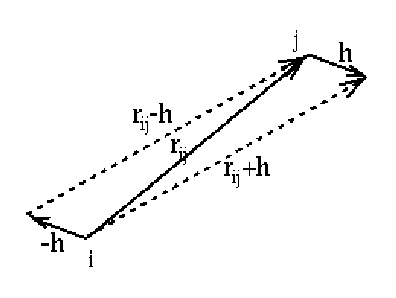
\epsfig{file=Implementation/vector_variation.eps, height=4cm}
  \caption{Addition of a vector at j equals the subtraction of the
  same vector at i}
  \label{vector_variation}
\end{center}
\end{figure}

As be can seen from figure \ref{vector_variation}\footnote{This is
  also easy to see from the relation $r_{ij} = \sqrt{
    \sum_{k=0}^{\bar{d}}(\xi_i^k-\xi_j^k)^2}$, 
where d is the number of dimensions, and $\bar{d}=d-1$.}, 

\begin{equation}
  r_{ij}(\xi_j+h) = r_{ij}(\xi_i-h)
\end{equation}

One object of class \emph{Distance} and 2d objects of class
\emph{DistanceDiff} holds all the information needed of the
inter-electronic distances for numerical calculation of both the
(centered difference) derivative and second derivative. Movement of
one electron consists of $(2d+1)\dot(N-1)$ updates of the distances,
and is thus of order ${\cal O}(N)$. Table \ref{Distance} give a list of the
public algorithms for the classes \emph{Distance} and
\emph{DistanceDiff}.

\begin{table}[hbtp]
\begin{center} {\large \bf Distance and DistanceDiff} \\ 
$\phantom{a}$ \\
\begin{tabular}{ll}
\hline\\ 
{\bf Algorithm}              & {\bf Usage} \\
Distance() or DistanceDiff() &Constructor\\
void attach(...)             &Attach intrinsic properties\\
void initialize()            &Initialize distances\\
void updateProposedMove()    &Calculate new distances for proposed move\\
void acceptMove()            &Accept proposed move\\
void rejectMove()            &Reject proposed move\\
double* getMatrix()          &Returns pointer to $rij$\\
double* getNewColumn()       &Returns pointer to $rij\_new\_column$\\
\hline
\end{tabular} 
\end{center}
\caption{Public algorithms for the classes Distance and DistanceDiff}
\label{Distance}
\end{table}

The differential parameters of
\emph{DistanceDiff}, $h$ and \emph{differentiate}, are assigned to
\emph{DistanceDiff} through the \emph{attach} algorithm. The value $h$
is the value added, or subtracted, to coordinate $differentiate$ of the
trial coordinate. \newline
An example on how to deal with upper triangular matrixes 
is in order. In the \emph{acceptMove} algorithm the new distances of
\emph{rij\_new\_column} is to be put into the upper-triangular matrix
$rij$. Here followes the \emph{acceptMove} algorithm:

{\footnotesize
\begin{enumerate}
\item[]
\begin{verbatim}
void Distance::acceptMove()
{
  __rij = rij-1+currentParticle;
  __rij_new_column = rij_new_column-1;
  int k=numParticles-1;
  for ( int i=0; i<currentParticle; i++ ) {
    (*__rij) = (*++__rij_new_column);
    k--;
    __rij+=k;
  }
  for ( int i=currentParticle+1; i<numParticles; i++)  
    (*++__rij)=(*++__rij_new_column);
  nextParticle();
}
\end{verbatim}

\end{enumerate}
}

For short we set $C=currentParticle$.
The pointer $\_\_rij$ is set to point at $r_{0C}$, if $C\ne
0$\footnote{If $C=0$ $\_\_rij$ is set to point at the element prior
  to the first element of $rij$},  
and $\_\_rij\_new\_column$ is set to point at the element
prior to the first element of $rij\_new\_column$\footnote{We
  create an extra element for this specific purpose.}.
Then we loop $i=0,C-1$, and set the value of $\_\_rij$ equal to the value
of the incremented $\_\_rij\_new\_column$, i.e. $r_{0C}$. We proceed
until $r_{\bar{C}C}$ (where $\bar{C}=C-1$). The pointer
$\_\_rij$ now points at $r_{\bar{C}\bar{N}}$, and in the
second loop it is incremented to point at $r_{CC^{^+}}$ (where $C^{^+}=C+1$),
and so is $\_\_rij\_new\_column$. Both pointers are incremented until
all the values are set, and we finally jump to the next particle.
\newline
Let us give an example of the $\_\_rij\_new\_column$ pointer. For $N=5$
and $C=2$ we have

\begin{equation}
  \begin{array}{cccccc}
  rij =
  |r_{01}, &r_{02}, \phantom{A} r_{03}, \phantom{A} r_{04}, &r_{12},
  \phantom{A} r_{13}, &r_{14}, &r_{23},
  &r_{24}, \phantom{A} r_{34}> \\
  pointer& \Uparrow \phantom{AAAAAAA}& \Uparrow \phantom{AAA}& \uparrow &
  \Uparrow & \Uparrow \phantom{AAAA}\\
  k& \phantom{AAA}3 & \phantom{AAAA}2 & \phantom{aa}1 & \phantom{aa}1 & 
  \end{array}
  \label{r_ij_array}
\end{equation}

We assign values at $\Uparrow$, and the $\uparrow$ is a temporary
pointer between the two loops.
This can more readily be seen by
looking at the corresponding matrix.

\begin{equation}
  r_{ij} = \left[
  \begin{array}{ccccc}
    0 & r_{01} & r_{02} & r_{03}  & r_{04}\\
    0 &   0    & r_{12} & r_{13}  & r_{14}\\
    0 &   0    &   0    & r_{23}  & r_{24}\\
    0 &   0    &   0    &   0     & r_{34}\\
    0 &   0    &   0    &   0     &   0   \\
  \end{array} \right]
\end{equation}

In the first loop we add one less than the number of none-zero
elements in the row we are at. Disregarding the none-zero elements,
this will take us to the element of the next row, with the same last index
(unless we are at the first element, in which case it will take us
to the last element).





%%%%%%%%%%%%%%%%%%%%% Jastrow and JastrowDiff %%%%%%%%%%%%%%%%%%%%
\subsection{Jastrow and JastrowDiff}

The classes \emph{Jastrow} and \emph{JastrowDiff} are similar to
\emph{Distance} and \emph{DistanceDiff}, respectively. First, they
contain information about the $f_{ij}$, in $f\_matrix$ (and the new
values for a proposed move, in \emph{f\_new\_column}). 
Furthermore, \emph{Jastrow} contains information about
the \emph{jastrowian}, $J$, and $\Delta J=J_{new}-J_{old}$.
Updating the $f_{ij}$'s for the jastrowian and its first and second
derivatives is also of order ${cal O}(N)$ (for the movement of one
electron).
Table \ref{Jastrow} lists the public algorithms of \emph{Jastrow} and
\emph{JastrowDiff}.

\begin{table}[hbtp]
\begin{center} {\large \bf Jastrow and JastrowDiff} \\ 
$\phantom{a}$ \\
\begin{tabular}{ll}
\hline\\ 
{\bf Algorithm}                        & {\bf Usage} \\
Jastrow() or JastrowDiff()             &  Constructor\\
void attach(...)                       &  Attach intrinsic properties\\
void initialize()                      &  Initialize the $f_{ij}$'s (and the jastrowian)\\
void updateProposedMove()              &Calculate new $f_{ij}$'s for proposed move\\
void acceptMove()                      &Accept proposed move\\
void rejectMove()                      &Reject proposed move\\
double* getFMatrix()                   &Returns pointer to $f\_matrix$\\
double* getFNewColumn()                &Returns pointer to $f\_new\_column$\\
void getFColumn(int i, double* fColumn)&Returns column i of $f\_matrix$ in fColumn\\
{\bf Jastrow-specific algorithms}      &\\
double\& operator()()                  &Returns the jastrowian, $J$\\
double getDifference()                 &Returns the difference, $\Delta J=J_{new}-J_{old}$\\
\hline
\end{tabular} 
 \end{center}
  \caption{Public algorithms for the classes Jastrow and JastrowDiff}
\label{Jastrow}
\end{table}

For example \emph{getFNewColumn} returns a pointer to:

\begin{equation}
  f\_new\_column = | f_{0i}, f_{1i}, \dots, f_{\bar{i}i}, f_{ii^{^+}},
  \dots, f_{i \bar{N}} >
\end{equation}

where $i$ is the current particle being moved.





%%%%%%%%%%%%%%%%%%%%% Derivatives %%%%%%%%%%%%%%%%%%%%
\subsection{Derivatives}

\emph{Derivatives} manages the derivatives of the $f_{ij}$'s. 
\newline
It is sufficient to calculate either $\frac{\delta f_{ij}}{\delta
  \xi_i}$ or $\frac{\delta f_{ij}}{\delta \xi_j}$, since 

\begin{equation}
  \frac{\delta f_{ij}}{\delta \xi_i} = \frac{\delta r_{ij}}{\delta \xi_i}
  \frac{d f_{ij}} {d r_{ij}} = - \frac{\delta r_{ij}}{\delta \xi_j}
  \frac{d f_{ij}} {d r_{ij}} = - \frac{\delta f_{ij}}{\delta \xi_j}
\end{equation}

In the above calculation we have used

\begin{equation}
  \frac{\delta r_{ij}}{\delta \xi_i^m} = \frac{\delta}{\delta \xi_i^m} 
  \sqrt{ \sum_{k=0}^{\bar{d}} (\xi_i^k-\xi_j^k)^2} =
  \frac{\xi_i^m-\xi_j^m}{r_{ij}} = - \frac{\delta
  r_{ij}}{\delta \xi_j^m} 
\end{equation}

where $\xi_i^m$ is cordinate $m$ of particle $i$, and $\bar{d}=d-1$. \newline
The upper triangular matrix:

\begin{equation}
  \frac{\delta f}{\delta \xi} = \left[
  \begin{array}{ccccc}
    0 & \frac{\delta f_{01}}{\delta \xi_1} & \frac{\delta
    f_{02}}{\delta \xi_2} & \dots & \frac{\delta f_{0\bar{N}}}{\delta
    \xi_{\bar{N}}} \\ 
    0 &        0        & \frac{\delta f_{12}}{\delta \xi_2} & \dots & 
    \frac{\delta f_{1\bar{N}}}{\delta \xi_{\bar{N}}} \\
    0 &        0        &          0            &\ddots &  \vdots       \\
    0 &        0        &          0            &   0   &
    \frac{\delta f_{\bar{\bar{N}}\bar{N}}}{\delta \xi_{\bar{N}}} \\
    0 &        0        &          0            &   0   &   0  
  \end{array} \right]
\label{df_dxi}
\end{equation}

is stored as an array, \emph{derivatives}, similar to that of
eq. (\ref{r_ij_array}). Also, we store 
the upper-triangular matrix of the second derivatives. The calculation
of the first derivative,

\begin{equation}
  \frac{\delta f_{ij}}{\delta \xi_i} \approx \frac{f_{ij}(\xi_i+h) -
  f_{ij}(\xi_i-h)}{2h} 
\end{equation}

and the second derivative,

\begin{equation}
  \frac{\delta^2 f_{ij}}{\delta \xi_i^2} \approx \frac{f_{ij}(\xi_i+h)
  + f_{ij}(\xi_i-h) - 2 f_{ij}}{h^2}
\end{equation}

uses the $f_{ij}$'s updated in \emph{Jastrow} and
\emph{JastrowDiff}. Movement of one particle involves
calculation of $N-1$ values of both $\frac{\delta f_{ij}}{\delta \xi_i}$
and $\frac{\delta^2 f_{ij}}{\delta \xi_i^2}$. Table \ref{Derivatives}
lists the public algorithms of \emph{Derivatives}.

\begin{table}[hbtp]
\begin{center} {\large \bf Derivatives} \\ 
$\phantom{a}$ \\
\begin{tabular}{ll}
\hline\\ 
{\bf Algorithm}                   & {\bf Usage} \\
Derivatives()                     &Constructor\\
void attach(...)                  &Attach intrinsic properties\\
void initialize()                 &Initialize the derivatives\\
void updateDerivatives()          &Calculate the new derivatives for a move\\ 
void acceptDerivatives()          &Updates the 1. and 2. derivatives matrix\\
void rejectDerivatives()          &Jumps to next particle without doing
anything\\
void getDColumn(int i, double* Column) 
  &Returns column i of $\frac{\delta f}{\delta \xi}$ in Column\\
double* getDNewColumn() &Returns pointer to new derivatives\\
void getD2Column(int i, double* Column)
  &Returns column i of $\frac{\delta^2 f}{\delta \xi^2}$ in Column\\
double* getD2NewColumn()&Returns pointer to new second derivatives\\
\hline
\end{tabular} 
 \end{center}
  \caption{Public algorithms for the class Derivatives}
\label{Derivatives}
\end{table}



%%%%%%%%%%%%%%%%%%%%% Correlation %%%%%%%%%%%%%%%%%%%%
\subsection{Correlation}

Before we proceed with the class structure, some theory must be
established. Let us start with the ratio
$\frac{G_{new}}{G_{old}}$, for the Metropolis algorithm. For $G=J$ we
have 

\begin{equation}
  \frac{G_{new}}{G_{old}} = \frac{J_{old}+\Delta J}{J_{old}}
\end{equation}

and for $G=e^J$,

\begin{equation}
  \frac{G_{new}}{G_{old}} = e^{\Delta J}
\end{equation}

$\nabla^2 J$ given by, 

\begin{equation}
  \nabla^2 J = \sum_{i=0}^{\bar{N}} \nabla_i^2 J =
  \sum_{i=0}^{\bar{N}} \nabla_i^2 \sum_{k<l} f_{kl} = 
  \sum_{i=0}^{\bar{N}} \left[ \sum_{k<l} \delta_{li} \nabla_i^2 f_{kl}
  + \sum_{k<l} \delta_{ki} \nabla_i^2 f_{kl} \right]
\end{equation}

where $\nabla_i^2 f_{ij} = \sum_{k=0}^{\bar{d}} \frac{\delta^2
  f_{ij}}{(\delta \xi_i^k)^2}$, and $\delta_{li}$ is the
Kronecker-delta. We define

\begin{equation}
  \nabla_i^2 J \equiv \sum_{j=0}^{i-1} \nabla_i^2 f_{ij}  +
  \sum_{j=i+1}^{\bar{N}} \nabla_j^2 f_{ij}
\end{equation}

and get 

\begin{equation}
  \nabla^2 J = \sum_{i=0}^{\bar{N}} \left[ \sum_{j=0}^{i-1} \nabla_i^2 f_{ij}
  + \sum_{j=i+1}^{\bar{N}} \nabla_i^2 f_{ij} \right] =
  \sum_{i=0}^{\bar{N}} \nabla_i^2 J
\end{equation}

from the relation $\nabla_i^2 f_{ij} = \nabla_j^2 f_{ij}$. If we move
one particle, $C$, all values in $\nabla^2_C J$, and one of the values
in $\nabla^2_i J$, $i\ne C$, are changed;

\begin{equation}
  \nabla_i^2 J^{new} = \nabla_i^2 J^{old} + \nabla_i^2 f_{iC}^{new} - \nabla_i^2 f_{iC}^{old}
\end{equation}

for all $i\ne C$, and

\begin{equation}
  \nabla_C^2 J^{new} = \sum_{i \ne C} \nabla_i^2 f_{iC}^{new}
\end{equation}

By changing only these values, we have an algorithm of order ${\cal O}(N)$
for the update of $\nabla^2 J$. \newline
For $\nabla J$, we have

\begin{equation}
  \nabla J = \left| \frac{\delta J}{\delta \xi_0^0},
  \dots , \frac{\delta J}{\delta \xi_{\bar{d}}^0}, \dots,
  \frac{\delta J}{\delta \xi_0^{\bar{N}}}, \dots, \frac{\delta J}{\delta
  \xi_{\bar{d}}^{\bar{N}}} \right>
\end{equation}

where

\begin{equation}
  \frac{\delta J}{\delta \xi^i} = \frac{\delta}{\delta \xi^i}
  \sum_{k<l} f_{kl} = \sum_{j=0}^{i-1} \frac{\delta f_{ji}}{\delta
  \xi^i}  + \sum_{j=i+1}^{\bar{N}} \frac{\delta f_{ij}}{\delta \xi^i} 
  = \sum_{j=0}^{i-1} \frac{\delta f_{ji}}{\delta
  \xi^i}  - \sum_{j=i+1}^{\bar{N}} \frac{\delta f_{ij}}{\delta \xi^j}
\end{equation}

since $\frac{\delta f_{ij}}{\delta \xi^i} = - \frac{\delta
  f_{ij}}{\delta \xi^j}$. 
All the values of the derivatives are kept
in the $d$ objects of class \emph{Derivatives}, and its easy to
calculate the above expression. However, we wish to keep the order of
our correlation routines as low as possible, so we follow a procedure
similar to that of $\nabla^2 J$;

\begin{equation}
  \frac{\delta J^{new}}{\delta \xi^i} = \frac{\delta J^{old}}{\delta
  \xi^i} + \frac{\delta f_{ji}^{new}}{\delta \xi^i} - \frac{\delta
  f_{ji}^{old}}{\delta \xi^i} 
\end{equation} 

for $i<C$,

\begin{equation}
  \frac{\delta J^{new}}{\delta \xi^i} = \frac{\delta J^{old}}{\delta
  \xi^i} - \frac{\delta f_{ji}^{new}}{\delta \xi^j} + \frac{\delta
  f_{ji}^{old}}{\delta \xi^j} 
\end{equation} 

for $i>C$, and for $C$

\begin{equation}
  \frac{\delta J^{new}}{\delta \xi^C} 
  = \sum_{j=0}^{C-1} \frac{\delta f_{jC}^{new}}{\delta
  \xi^C}  - \sum_{j=C+1}^{\bar{N}} \frac{\delta f_{Cj}^{new}}{\delta \xi^j}
\end{equation}

For $G=J$ we can use the above relations directly. For $G=e^J$ a few
minor modifications must be made:

\begin{equation}
  \nabla e^J = \nabla J \dot e^J
\end{equation}

and

\begin{equation}
  \nabla^2 e^J = \nabla (\nabla J \dot e^J) = \left[ \nabla^2 J +
  (\nabla J)^2  \right] e^J
\end{equation}

I.e. $e^J$, $\nabla J$ and $\nabla^2 J$ holds all the information needed to
compute $\nabla e^J$ and $\nabla^2 e^J$. The above computations are
also of the order ${\cal O}(N)$. \newline


\emph{Correlation} is the class used by the VMC-algorithm to manage
all information 
about the correlation. It is used to calculate the gradient, and the
gradient squared, of the correlation. Also, the ratio
$\frac{G_{new}}{G_{old}}$ for a proposed move is calculated, as well
as the value of the correlation, $G$, itself. Routines for both
thermalization- and VMC-moves are implemented. \newline
Table \ref{Correlation} lists the public algorithms of \emph{Correlation}.

\begin{table}[hbtp]
\begin{center} {\large \bf Correlation} \\ 
$\phantom{a}$ \\
\begin{tabular}{ll}
\hline\\ 
{\bf Algorithm}                 & {\bf Usage} \\
Derivatives(Domain\& domain)    &Constructor\\
void proposeMove()              &Updates the values (in the Jastrow and
Distance objects)\\
 & needed to determine the ratio $\frac{G_{new}}{G_{old}}$\\
void initializeThermalizedMove()&Initializes the Jastrow and Distance objects\\
void acceptThermalizedMove()    &Updates the Jastrow and Distance objects\\
void rejectThermalizedMove()    &Jumps to next particle without doing anything\\
void initializeVMC()            &Initializes the JastrowDiff, DistanceDiff 
              and Derivatives\\ 
&objects, and initializes $\nabla G$ and $\nabla^2 G$\\
void acceptVMCMove()            &Update $\nabla G$ and $\nabla^2 G$,
and updates the Jastrow, JastrowDiff,\\
& Distance, DistanceDiff and Derivatives objects\\
void rejectVMCMove()            &Jumps to next particle without doing anything\\
double operator()()             &Returns the correlation, $G$,
i.e. either $J$ or $e^J$\\
double getRatio()               &Returns the ratio $\frac{G_{new}}{G_{old}}$\\
double* getGradient()           &Returns pointer to $\nabla G$\\
double getGrad2()               &Returns the value of $\nabla^2 G$\\
\hline
\end{tabular} 
 \end{center}
  \caption{Public algorithms for the class Correlation}
\label{Correlation}
\end{table}

The constructor uses the \emph{Domain} class to access information
about properties like the number of particles $N$, the number of
dimensions $d$, and all the coordinates. The \emph{proposeMove}
algorithm updates the changes in the jastrowian due to a proposed move
in the trial coordinate. Furthermore, it stores the
new inter-electronic distances, and the new $f_{ij}$'s in two arrays;
\emph{rij\_new\_column} in the object of class\emph{Distance} and
\emph{f\_new\_column} in the object of class \emph{Jastrow}. \newline 
If the move is accepted, the values of the differences must be
updated, as well as the derivatives and the gradients (for a VMC
move\footnote{In the case of thermalization, no
  sample of the energy is preformed, so no derivatives (or
  differences) are calculated.}). 
In the \emph{acceptVMCmove} algorithm, see table \ref{Correlation}, the
values of $\nabla J$ and $\nabla^2 J$ are calculated. $\nabla G$
and $\nabla^2 G$ are not calculated until the \emph{getGradient} and
\emph{getGrad2} routines.
Finally, all new values must be assigned to their respective
upper-triangular matrices, before we proceed to the next particle. 
\newline
If the move is not accepted, we simply proceed to the next particle,
without performing any changes.



%%%%%%%%%%%%%%%%%%%%% CoorExt %%%%%%%%%%%%%%%%%%%%
\subsection{CoorExt}

The class \emph{CoorExt}, defined in \emph{Coor.h}, manages the
particles coordinates. Table 
\ref{CoorExt} lists the public algorithms of \emph{CoorExt}. 

\begin{table}[hbtp]
\begin{center} {\large \bf CoorExt} \\ 
$\phantom{a}$ \\
\begin{tabular}{ll}
\hline\\ 
{\bf Algorithm}                   & {\bf Usage} \\
CoorExt()                         & Empty constructor\\
CoorExt(double* x, int \_len,     & Constructor\\
\phantom{a} int \_\_spin, double* \_ext)& \\
void attach(double* \_\_x, int \_len,& Attaches intrinsic properties\\
\phantom{a} int \_\_spin, double* \_ext)& \\
double\& operator()()             & Returns the current cartesian coordinate\\
double\& operator()(int num)      & Returns coordinate num\\
void operator++(int)              & Increments pointer to next cartesian coordinate\\
void resetPtr                     & Resets pointer to first cartesian coordinate\\
int getLen()                      & Returns the number of cartesian coordinates\\
double r()                        & Returns the distance form the nucleus\\
void calculateR()                 & Computes the distance to the nucleus\\
int\& spin()                      & Returns the electron eigen-spin\\
int flipSpin()                    & Returns negative multiple of spin\\
double param(int i)               & Returns the value of parmeter number i; ext[i]\\
\hline
\end{tabular} 
 \end{center}
  \caption{Public algorithms for the class CoorExt}
\label{CoorExt}
\end{table}

\emph{CoorExt} contains all the information needed of each electron;
its cartesian coordinates and its eigen-spin. Furthermore, it contains
a pointer to the variational parameters of the Slater determinant
orbital wave-functions. In this manner one orbital function may be
computed directly given one \emph{CoorExt} object.
Also, the electron distance from the origin is calculated, and it
allows a spin flip.



%%%%%%%%%%%%%%%%%%%%% FuncSetMultivar %%%%%%%%%%%%%%%%%%%%
\subsection{FuncSetMultivar}

The class \emph{FuncSetMultivar}, defined in \emph{Func.h}, manages a
set of functions and their 
derivatives. Each column in a Slater matrix is represented as one such
object. Table \ref{FuncSetMultivar} lists some\footnote{All the
  \emph{attach} procedures are left out, Furthermore, most of the
  algorithms are implemented twice; ($\dots$) means either with or
  without an input (\emph{Param\& \_coordinate}).} of the public algorithms
of \emph{FuncSetMultivar}.

\begin{table}[hbtp]
\begin{center} {\large \bf FuncSetMultivar} \\ 
$\phantom{a}$ \\
\begin{tabular}{ll}
\hline\\ 
{\bf Algorithm}                   & {\bf Usage} \\
FuncSetMultivar($\dots$)          & Constructor\\
void init($\dots$)                & Initialize intrinsic properties\\
void calcValueCenter($\dots$)     & Calculates the function values (given coordinate)\\
void calcValueSides($\dots$)      & Calculates the function values (given differentiated coordinate)\\

double valuePt()                  & Returns pointer to different calculated values\\
double diff()                     & Calculates the first derivatives\\
double diff(int v)                & Calculates the first derivatives
with respect to the\\
                                  & indexed variable (of all functions)\\
double ddiff()                    & Calculates the second derivatives\\
\hline
\end{tabular} 
 \end{center}
  \caption{Public algorithms for the class FuncSetMultivar}
\label{FuncSetMultivar}
\end{table}

In order to find the derivatives of the functions for a given
coordinate, \emph{calcValueCenter} and \emph{calcValueSides}
must be called prior to \emph{diff}. The second derivatives are
calculated with a call to the \emph{ddiff} algorithm.



%%%%%%%%%%%%%%%%%%%%% Functor %%%%%%%%%%%%%%%%%%%%
\subsection{Functor}

The template class \emph{Functor} defines a functor. 
We have chosen to use a functor-type object, to increase
flexibility, and have the ability to use more complex functions
later without changing too much code\footnote{This is good programming
  philosophy; we may want to improve the program at a later stage.}.
Table \ref{Functor} lists the public algorithm of \emph{Functor}.

\begin{table}[hbtp]
\begin{center} {\large \bf Functor} \\ 
$\phantom{a}$ \\
\begin{tabular}{ll}
\hline\\ 
{\bf Algorithm}                   & {\bf Usage} \\
Functor()                         & Empty constructor\\
Functor(Function\& \_function)    & Constructor\\
void attach(Function\& \_function)& Attaches a function\\
Return operator()(Param\& coor)   & Returns an object of type Return\\
\hline
\end{tabular} 
 \end{center}
  \caption{Public algorithms for the class Functor}
\label{Functor}
\end{table}


Given an argument 
\emph{Param} the functor returns \emph{Return}. Both \emph{Param} and
\emph{Return} are classes, e.g. \emph{double}, \emph{CoorExt} etc.
To give an example, we can create a functor with the call:

{\footnotesize
\begin{enumerate}
\item[]
  \begin{verbatim}
Functor<CoorExt, double>* function;
function = new Functor<CoorExt, double>();
\end{verbatim}

\end{enumerate}
}

We need some formula for calculating the return value of type
\emph{double}, given an object of class \emph{CoorExt}. If we first
define the function \emph{hydr1s} given by:

{\footnotesize
\begin{enumerate}
\item[]
  \begin{verbatim}
double hydr1s(CoorExt& coordinate) {
  return exp(- coordinate.param(0) * coordinate.r());
}
\end{verbatim}

\end{enumerate}
}

and then attach it to the \emph{Functor} object \emph{function}:

{\footnotesize
\begin{enumerate}
\item[]
  \begin{verbatim}
function[0].attach(hydr1s);
\end{verbatim}

\end{enumerate}
}

We may then calculate the value of the function with the call:

{\footnotesize
\begin{enumerate}
\item[]
  \begin{verbatim}
function_value = (function[0])(coordinate);
\end{verbatim}

\end{enumerate}
}

where \emph{coordinate} is an object of class \emph{CoorExt}. 



%%%%%%%%%%%%%%%%%%%%% Random %%%%%%%%%%%%%%%%%%%%
\subsection{Random}

The two classes \emph{Ran0} and \emph{Ran1}, in
\emph{Random.h}, defines the random generators used by the
Metropolis random movement. We want our electrons to move \emph{randomly}
in space, and at the same time we want to reduce the CPU-time of our
calculations. Therefore, the program should be tested with different
random generators. Table \ref{Random} lists the
public algorithms of the random generators.

\begin{table}[hbtp]
\begin{center} {\large \bf Random} \\ 
$\phantom{a}$ \\
\begin{tabular}{ll}
\hline\\ 
{\bf Algorithm}                   & {\bf Usage} \\
Ran0(long seed) or Ran1(long seed)& Constructor\\
double getNum(void)               & Returns double in the range (0,1]\\
\hline
\end{tabular} 
 \end{center}
  \caption{Public algorithms for the class Random}
\label{Random}
\end{table}

We will not get into the details of the random generators, and simply
refere to \emph{???reference here???}. However, of importance to the
user is the integral seed. This seed is changed with each call to
\emph{getNum}. Giving the same seed twice produces the exact same
number, and if called several times they will produce the same
sequences of numbers. To produce indepentent runs, the seed
must differ with each run\footnote{An other problem may also
  arise. Even with two different seeds, one of the sequences may by
  chance produce the other seed, and thereby produce the same sequence
following this number. This problem will not be addressed in this
scope, but note that this chance is extremely small, and given two
different starting positions, the Metropolis algorithm should not
become too biased even if this were to occur.}












































%\documentclass[../main.tex]{subfiles}
 
\begin{document}

\chapter{Results}\label{sec: Results}

Natural units ($\hbar=c=e=m_e=1$) were used to obtain all the results listed in this chapter.

\section{Optimization}

Here we look at the effect that various optimizations had on the computation time of our program. The optimization to the simulation itself gave a total speed-up factor of $31.246$ for the tested system, while running the program in parallel on $4$ processors gave an additional speed-up factor of around $3.6$.

\subsection{Storing Reused Data and Optmizing Hermite Polynomials}

For the following optimization results we used a system of two particles in a two-dimensional double harmonic oscillator well as reference system. For the results in Table \ref{tab: OptimizationExpansion} we used $465$ basis functions. From the table we see that including the "-ffast-math" compiler flag gives a decent speed up, but the storing of the Slater related matrices and the efficient computation of Hermite polynomials are the most important optimizations in this case. We also see that the "-ffast-math" flag is much more important when we include the Hermite optimization described in Section \ref{sec:Optimizing Hermite}. In this case the storing of the relative distances and the Jastrow related matrices, provide seemingly no speed up. This makes sense since these optimizations scale well with the number of particles used, and therefore become important for large numbers of particles. In our case we only have two particles so the effect of these optimizations is negligible. The optimization of Hermite polynomial calculation obviously scales with the number of Hermite polynomials we need. The number of Hermite polynomials we need scales with the number of basis functions we use, and in our case we use $465$ basis functions, which means we need the first $30$ Hermite polynomials, each of which has to be calculated many times for various positions of particles. The efficiency gain from storing the Slater related matrices also scales with the number of basis functions. This is because these matrices store the single particle wave functions and their derivatives. These single particle wave functions are calculated by a loop over the number of basis functions, so if we avoid recalculating them unnecessarily, we reduce the number of basis function loops, which of course is more important if we use a lot of basis functions.

\begin{table}[!ht]
  \centering
  \begin{tabular}{ | c | c | c | c |}
    \hline
    Optmizations & Avg. Time [s] & Speed Up & Total Speed Up\\*
    \hline
    B & 122.173 & 1.000 & 1.000\\*
    \hline
    B F & 104.244 & 1.172 & 1.172\\*
    \hline
    B F D & 104.296 & 1.000 & 1.171\\*
    \hline
    B F D S & 16.8304 & 6.197 & 7.259\\*
    \hline
    B F D S J & 16.8524 & 0.999 & 7.250\\*
    \hline
    B F D S J H & 3.91007 & 4.310 & 31.246\\*
    \hline
    B D S J H & 30.7192 & 0.127 & 4.017\\*
    \hline
  \end{tabular}
  \caption{Optimization results for two particles in a two-dimensional double harmonic oscillator well. The number of basis functions used was $465$. The letter B stands for base i.e. the program before doing optimizations. The letter F is for using the "-ffast-math" compiler flag, D is for storing the distance matrix, S is for storing the Slater related matrices, J is for storing the Jastrow related matrices, and H is for optimal computation of Hermite polynomials. The "Avg. Time" column is the average time over five runs, the "Speed Up" column lists the speed up factor relative to the row above, and the "Total Speed Up" column lists the speed up factor relative to the first row. Optimizations D and J have seemingly no effect on the run-time, because they scale with the number of particles and we only use two particles in this case. The gain from using the F optimization is much greater when we also use the H optimization. This is apparent by comparing the first two rows with the last two rows. The S and H optimizations provide the most speed up for this system.}
  \label{tab: OptimizationExpansion}
\end{table}

%\begin{table}[!ht]
%  \centering
%  \begin{tabular}{ | c | c | c | c | c | c | c | c | c |}
%    \hline
%    Optmizations & Run 1 & Run 2 & Run 3 & Run 4 & Run 5 & Avg. & Speed Up & Total\\*
%    \hline
%    B & 122.074 & 122.730 & 122.223 & 122.006 & 121.834 & 122.173 & 1.000 & 1.000\\*
%    \hline
%    B F & 104.236 & 104.029 & 103.951 & 104.515 & 104.489 & 104.244 & 1.172 & 1.172\\*
%    \hline
%    B F D & 103.960 & 104.523 & 104.207 & 104.359 & 104.429 & 104.296 & 1.000 & 1.171\\*
%    \hline
%    B F D S & 16.8619 & 16.6298 & 16.9949 & 16.8100 & 16.8552 & 16.8304 & 6.197 & 7.259\\*
%    \hline
%    B F D S J & 16.8360 & 16.9138 & 17.0127 & 16.8403 & 16.6593 & 16.8524 & 0.999 & 7.250\\*
%    \hline
%    B F D S J H & 3.99471 & 3.87888 & 3.89648 & 3.74037 & 4.03992 & 3.91007 & 4.310 & 31.246\\*
%    \hline
%    B D S J H & 30.8744 & 30.7226 & 30.8116 & 30.7741 & 30.4132 & 30.7192 & 0.127 & 4.017\\*
%    \hline
%  \end{tabular}
%  \caption{}
%  \label{tab: OptimizationExpansion}
%\end{table}

In order to see that storing the distances and the Jastrow related matrices do actually contribute to the optimization, we will look at a different system. We now look at a system of $24$ particles in a two-dimensional double harmonic oscillator well. However, we now approximate the single particle wave functions with super positions of two harmonic oscillator functions, similarly to what was done in Chapter 5.1.3 and 5.2.3 of Ref. \cite{Jorgen}. This means that the number of Hermite calculations needed is significantly reduced, and the effect of storing the distances and the Jastrow related matrices should stand out due to the increased number of particles. Note that this way of calculating the single particle wave functions is not the focus of this thesis, but it has been implemented in order to compare the results of the two methods. In this case we use this method in order to simulate $24$ particles with reasonably short run times, as this method is generally faster especially for large number of particles. The benefit of storing the distances and the Jastrow related matrices should be similar for both methods, since the difference between them is how the single particle wave functions are calculated, and these single particle wave functions do not depend on the Jastrow factor or the distances between particles. The optimization results for this system are listed in Table \ref{tab: OptimizationSupPos}. As expected the importance of storing the distances and the Jastrow related matrices has gone up. The storing of distances provide a decent speed up, while the storing of the Jastrow related matrices is in this case the most important optimization. The storing of the Slater related matrices is not quite as important as it was in Table \ref{tab: OptimizationExpansion}, but it still provides a pretty good speed up. The effect of using the "-ffast-math" flag is much smaller in this case, and the effect of calculating Hermite polynomials is negligible. This method needs a lot less Hermite polynomial calculations, since there is no loop over basis functions when calculating the single particle wave functions. However, the number of Hermite polynomial calculations does scale with the number of particles, and the recursive method becomes slow for large numbers of particles, so for systems with even more particles the Hermite optimization should become significant for this method as well.

\begin{table}[!ht]
  \centering
  \begin{tabular}{| c | c | c | c |}
    \hline
    Optmizations & Avg. Time [s] & Speed Up & Total Speed Up\\*
    \hline
    B & 103.576 & 1.000 & 1.000\\*
    \hline
    B F & 101.766 & 1.018 & 1.018\\*
    \hline
    B F D & 92.2338 & 1.103 & 1.123\\*
    \hline
    B F D S & 54.7138 & 1.686 & 1.893\\*
    \hline
    B F D S J & 10.7135 & 5.107 & 9.668\\*
    \hline
    B F D S J H & 10.6977 & 1.001 & 9.682\\*
    \hline
    B D S J H & 10.8811 & 0.983 & 9.519\\*
    \hline
  \end{tabular}
  \caption{Optimization results for $24$ particles in a two-dimensional double harmonic oscillator well. The letter B stands for base i.e. the program before doing optimizations. The letter F is for using the "-ffast-math" compiler flag, D is for storing the distance matrix, S is for storing the Slater related matrices, J is for storing the Jastrow related matrices, and H is for optimal computation of Hermite polynomials. The "Avg. Time" column is the average time over five runs, the "Speed Up" column lists the speed up factor relative to the row above, and the "Total Speed Up" column lists the speed up factor relative to the first row. The single particle wave functions were approximated by a super position of two harmonic oscillator functions instead of the method regularly used in this thesis. The method used here involves less Hermite polynomial calculations, and as a result, optimizing the calculation of Hermite polynomials is less important. The benefit of optimizations D and J should be similar between the methods, and now that the number of particles is increased the effect of these optimizations is also increased compared to Table \ref{tab: OptimizationExpansion}. Optimazation D now provides a decent speed up, while optimization J provides the majority of the total speed up. Optimization S also provides a good speed up, but it is not as significant as it was in Table \ref{tab: OptimizationExpansion}.}
  \label{tab: OptimizationSupPos}
\end{table}

%\begin{table}[!ht]
%  \centering
%  \begin{tabular}{ | c | c | c | c | c | c | c | c | c |}
%    \hline
%    Optmizations & Run 1 & Run 2 & Run 3 & Run 4 & Run 5 & Avg. & Speed Up & Total\\*
%    \hline
%    B & 103.804 & 103.122 & 103.119 & 104.314 & 103.523 & 103.576 & 1.000 & 1.000\\*
%    \hline
%    B F & 101.842 & 100.080 & 99.9448 & 100.403 & 106.561 & 101.766 & 1.018 & 1.018\\*
%    \hline
%    B F D & 91.8727 & 91.5986 & 94.2381 & 91.8457 & 91.6137 & 92.2338 & 1.103 & 1.123\\*
%    \hline
%    B F D S & 54.4560 & 55.5666 & 54.3716 & 54.3464 & 54.8286 & 54.7138 & 1.686 & 1.893\\*
%    \hline
%    B F D S J & 10.6361 & 10.9981 & 10.6575 & 10.7927 & 10.4832 & 10.7135 & 5.107 & 9.668\\*
%    \hline
%    B F D S J H & 10.5354 & 10.7410 & 10.9612 & 10.7303 & 10.5204 & 10.6977 & 1.001 & 9.682\\*
%    \hline
%    B D S J H & 10.8578 & 10.8000 & 10.8382 & 10.8467 & 11.0629 & 10.8811 & 0.983 & 9.519\\*
%    \hline
%  \end{tabular}
%  \caption{}
%  \label{tab: OptimizationSupPos}
%\end{table}

\subsection{Parallelization}

As discussed in Section \ref{sec:Parallel}, the variational Monte Carlo (VMC) simulation can be parallelized without mid-simulation communication between the processors. Therefore we can expect near linear scaling, so doubling the number of processors should about halve the run time. In Table \ref{tab: Parallel1} we have listed average run times for a system of two particles in a two-dimensional double harmonic oscillator well, when using $1275$ basis functions and $1$, $2$ and $4$ processors. From the table we see that the speed up is close to what we expect, but not quite. 

\begin{table}[!ht]
  \centering
  \begin{tabular}{| c | c | c | c |}
    \hline
    Processors & Avg. Time [s] & Speed Up & Total Speed Up\\*
    \hline
    1 & 36.9145 & 1.0000 & 1.0000\\*
    \hline
    2 & 19.1713 & 1.9255 & 1.9255\\*
    \hline
    4 & 10.3109 & 1.8593 & 3.5801\\*
    \hline
  \end{tabular}
  \caption{Parallelization results for two particles in a two-dimensional double harmonic oscillator well. The number of basis functions used was $1275$. The "Avg. Time" column is the average time over five runs, the "Speed Up" column lists the speed up factor relative to the row above, and the "Total Speed Up" column lists the speed up factor relative to the first row. We see that doubling the number of processors gives a speed up factor close to $2$, but it is still somewhat off, especially when going from $2$ to $4$ processors.}
  \label{tab: Parallel1}
\end{table}

A possible reason for why the results in Table \ref{tab: Parallel1} were somewhat different than expected could be that the run times were so short that the parallel overhead\footnote{Parallel overhead is the amount of time required to coordinate parallel tasks, as opposed to doing useful work. This can include factors such as: start-up time, synchronizations, data communications, software overhead imposed by libraries, operating system, etc., and termination time.\cite{Blaise}} was responsible for a significant fraction of the run time. If this is the case, doing the same test for a system that requires more CPU time, should provide results closer to the near linear scaling we expect. We increase the number of particles to $4$, and the run times for this system are listed in Table \ref{tab: Parallel2}. We end up with run times which are about three times as long as for the previous system, and as expected the speed up from parallelization is indeed somewhat greater for this system than for the two-particle system.

\begin{table}[!ht]
  \centering
  \begin{tabular}{| c | c | c | c |}
    \hline
    Processors & Avg. Time [s] & Speed Up & Total Speed Up\\*
    \hline
    1 & 107.468 & 1.0000 & 1.0000\\*
    \hline
    2 & 55.4418 & 1.9384 & 1.9384\\*
    \hline
    4 & 29.4316 & 1.8838 & 3.6514\\*
    \hline
  \end{tabular}
  \caption{Parallelization results for $4$ particles in a two-dimensional double harmonic oscillator well. The number of basis functions used was $1275$. The "Avg. Time" column is the average time over five runs, the "Speed Up" column lists the speed up factor relative to the row above, and the "Total Speed Up" column lists the speed up factor relative to the first row. We see that doubling the number of processors gives a speed up factor close to $2$, and the speed up factor are closer to $2$ in this case than they were in Table \ref{tab: Parallel1}. This is likely due to the generally longer run times for this system compared to the two-particle system. Since the run time is longer, the overhead is a smaller percentage of the total run time, which means it has less of an effect on the speed up factors.}
  \label{tab: Parallel2}
\end{table}

\section{Single Harmonic Oscillator Well}

In this section we look at the energy and one-body density of systems of particles in a single harmonic oscillator potential well, both in two and three dimensions.

\subsection{Ground State Energies}\label{sec: SHO GSE}

Here we look at the ground state energies for systems with various $\omega$ and number of particles. The ground state energies are calculated with the single particle wave functions being approximated by expansion in a single harmonic oscillator basis, and also by using harmonic oscillator single particle wave functions directly. Since the wave functions we are trying to approximate and the basis functions we use are of the same type (single harmonic oscillator) we should expect the two methods to yield the exact same results using a small amount of basis functions, just as we saw for the non-interacting case in Section \ref{sec:testSHO}. It turns out that we do not get the exact same results for the interacting case, however the same results are achieved if the variational parameter $\alpha$ is kept constant at $\alpha = 1$, while the other variational parameter $\beta$ is varied as usual. This indicates that there is an $\alpha$ dependence in the coefficients used in the basis function expansion, which our method fails to include. This $\alpha$ dependence could be included by doing a Hartree-Fock calculation on the coefficients, and this would be the next step in improving the method, but has not been done in this thesis.

\subsubsection{Two Dimensions}

The ground state energies for the two-dimensional case are listed in Table \ref{tab: EnergiesSHO2D}. The energies $E_\textrm{coeff}$ are the results when the single particle wave functions are approximated by expansion in a single harmonic oscillator basis, while $E_\textrm{reg}$ are the results when using harmonic oscillator single particle wave functions directly. We see from the table that $E_\textrm{coeff}$ and $E_\textrm{reg}$ are similar, especially for small numbers of particles $N$, but they are not exactly equal. Some further calculations not included here, revealed that the exact same energies where achieved if $\alpha$ was held constant at $\alpha = 1$, and $\beta$ was treated as the only variational parameter. This indicates that there is an $\alpha$ dependence in the coefficients used in the basis function expansion, which is not included when creating the coefficients. The coefficients could be modified to include this $\alpha$ dependence by doing a Hartree-Fock calculation, and if this is done $E_\textrm{coeff}$ and $E_\textrm{reg}$ should be exactly equal. 

The results $E_\textrm{coeff}$ and $E_\textrm{reg}$ are also bench-marked against results from various other methods such as Coupled Cluster and Full Configuration Interaction, as well as other VMC results. From Ref.~\cite{Taut} we also have an analytical result for the ground state energy, $E=3$, for the two-body case with $\omega=1$. The results are reasonably consistent with the benchmarks for all calculated systems. Our $E_\textrm{reg}$ results and the $E_\textrm{ref}^\textrm{(a)}$ benchmarks use the same VMC method, and as such should give fairly similar results. However, the optimization of parameters is done using different methods, which can result in slightly different parameter values being used, which in turn can result in differences larger than the statistical error. If the parameters used were exactly the same there could still be differences due to different amount of Monte Carlo cycles used, but in that case the statistical error would cover the difference. Table \ref{tab: DMCEnergiesSHO2D} has additional benchmarks from using Diffusion Monte Carlo, which is an improved version of VMC. Expanding our program to include DMC calculation as well as using Hartree-Fock to improve the coefficients is a possibility for further work.

\begin{table}[!ht]
  \centering
  \begin{tabularx}{\textwidth}{@{}ccYYYYYY@{}}%{ c c c c c c c c }
    \hline
    \hline
    $N$ & $\omega$ & $E_\textrm{coeff}$ & $E_\textrm{reg}$ & $E_\textrm{ref}^\textrm{(a)}$ & $E_\textrm{ref}^\textrm{(b)}$ & $E_\textrm{ref}^\textrm{(c)}$ & $E_\textrm{ref}^\textrm{(d)}$ \\*
    \hline
    2  & 0.01 & 0.0754(3) & 0.0745(2) & 0.07406(5) & - & 0.0738 \{23\} & 0.07383505 \{19\} \\*
       & 0.10 & 0.4460(3) & 0.4428(2) & 0.44130(5) & - & 0.4408 \{23\} & 0.44079191 \{19\} \\*
       & 0.28 & 1.0283(3) & 1.0245(3) & 1.02215(5) & - & 1.0217 \{23\} & 1.0216441 \{19\} \\*
       & 0.50 & 1.6658(3) & 1.6614(4) & 1.66021(5) & - & 1.6599 \{23\} & 1.6597723 \{19\} \\*
       & 1.00 & 3.0034(4) & 2.9984(4) & 3.00030(5) & - & 3.0002 \{23\} & 3.0000001 \{19\} \vspace{2 mm}\\*
    
    6  & 0.10 & 3.602(3) & 3.565(2) & 3.5690(3) & 3.49991 \{18\} & 3.5805 \{22\} & 3.551776 \{9\} \\*
       & 0.28 & 7.658(3) & 7.609(2) & 7.6216(4) & 7.56972 \{18\} & 7.6254 \{22\} & 7.599579 \{6\}  \\*
       & 0.50 & 11.853(3) & 11.781(2) & 11.8103(4) & 11.76228 \{18\} & 11.8055 \{22\} & 11.785915 \{6\} \\*
       & 1.00 & 20.243(3) & 20.143(3) & 20.1902(4) & 20.14393 \{18\} & 20.1734 \{22\} & 20.160472 \{8\} \vspace{2 mm}\\*
    
    12 & 0.10 & 12.568(7) & 12.282(3) & 12.3162(5) & 12.22533 \{17\} & 12.3497 \{21\} & 12.850344 \{3\} \\*
       & 0.28 & 25.866(6) & 25.642(4) & 25.7015(6) & 25.61084 \{17\} & 25.7095 \{21\} & 26.482570 \{2\} \\*
       & 0.50 & 39.406(5) & 39.152(4) & 39.2343(6) & 39.13899 \{17\} & 39.2194 \{21\} & 39.922693 \{2\} \\*
       & 1.00 & 65.952(5) & 65.666(4) & 65.7905(7) & 65.68304 \{17\} & 65.7399 \{21\} & 66.076116 \{3\} \\*
    \hline
    \hline
  \end{tabularx}
  \caption{The table lists ground state energy results for various single harmonic oscillator systems in two dimensions, and corresponding benchmarks. $N$ is the number of particles and $\omega$ is the harmonic oscillator frequency. $E_\textrm{coeff}$ are the energies obtained when the single particle wave functions are approximated by expansion in a single harmonic oscillator basis. For this the number of basis functions used was $(N/2)(N/2+1)/2$. $E_\textrm{reg}$ are the energies obtained when using harmonic oscillator single particle wave functions directly. The benchmarks are from the following: (a) J. Høgberget \cite{Jorgen} (VMC), (b) S. Reimann \cite{Reimann} (Similarity Renormalization Group theory), (c): C. Hirth \cite{Hirth} (Coupled Cluster Singles and Doubles), (d): V. K. B. Olsen \cite{Olsen} (Full Configuration Interaction). The numbers in parenthesis are the statistical errors found using blocking. In the curly brackets are the numbers of shells used above the last filled shell to construct the basis for the corresponding methods \cite{Jorgen}.}
  \label{tab: EnergiesSHO2D}
\end{table}

\begin{table}[!ht]
  \centering
  \begin{tabular}{c c c c}
    \hline
    \hline
    $N$ & $\omega$ & $E_\textrm{ref}^\textrm{(a)}$ & $E_\textrm{ref}^\textrm{(b)}$ \\*
    \hline
    2 & 0.01 & - & 0.073839(2) \\*
      & 0.10 & - & 0.44079(1) \\*
      & 0.28 & - & 1.02164(1) \\*
      & 0.50 & 1.65975(2) & 1.65977(1) \\*
      & 1.00 & 3.00000(3) & 3.00000(3) \vspace{2 mm}\\*
      
    6 & 0.10 & - & 3.55385(5) \\*
      & 0.28 & 7.6001(1) & 7.60019(6) \\*
      & 0.50 & 11.7888(2) & 11.78484(6) \\*
      & 1.00 & 20.1597(2) & 20.15932(8) \vspace{2 mm}\\*
      
    12 & 0.10 & - & 12.26984(8) \\*
       & 0.28 & 25.6356(1) & 25.63577(9) \\*
       & 0.50 & 39.159(1) & 39.1596(1) \\*
       & 1.00 & 65.700(1) & 65.7001(1) \\*
    \hline
    \hline
  \end{tabular}
  \caption{The table lists additional benchmarks for Table \ref{tab: EnergiesSHO2D}. $N$ is the number of particles and $\omega$ is the harmonic oscillator frequency. The benchmarks are from the following: (a) M. L. Pedersen et al. \cite{QDotBenchmarks} (DMC), (b) J. Høgberget \cite{Jorgen} (DMC).}
  \label{tab: DMCEnergiesSHO2D}
\end{table}

\subsubsection{Three Dimensions}

For the three-dimensional case the ground state energy results are listed in Table \ref{tab: EnergiesSHO3D}. Here we only have one source of benchmarks, but with both VMC and DMC benchmarks. From the table we mainly see the same things as for the two-dimensional case. The results are reasonably consistent with the benchmarks and with each other. By looking at the two particle case we can see that in general the energy is larger in three dimensions than in two dimensions for the same system, but the difference is smaller for smaller $\omega$. For $E_\textrm{reg}$ and $\omega = 0.01$ the ratio is $0.0790/0.0745 \approx 1.0604$, while for $\omega = 1$ it is $3.7242/2.9984 \approx 1.2421$.

\begin{table}[!ht]
  \centering
  \begin{tabularx}{\textwidth}{@{}ccYYYY@{}}%{ c c c c c c c c }
    \hline
    \hline
    $N$ & $\omega$ & $E_\textrm{coeff}$ & $E_\textrm{reg}$ & $E_\textrm{ref}^\textrm{(a)}$ & $E_\textrm{ref}^\textrm{(b)}$ \\*
    \hline
    2 & 0.01 & 0.0800(2) & 0.0790(1) & 0.07939(3) & 0.079206(3) \\*
      & 0.10 & 0.5004(2) & 0.4993(3) & 0.50024(8) & 0.499997(3) \\*
      & 0.28 & 1.2006(2) & 1.1993(3) & 1.20173(5) & 1.201725(2) \\*
      & 0.50 & 1.9977(2) & 1.9963(3) & 2.00005(2) & 2.000000(2) \\*
      & 1.00 & 3.7257(3) & 3.7242(3) & 3.73032(8) & 3.730123(3) \vspace{2 mm}\\*
      
    8 & 0.10 & 5.726(2) & 5.699(2) & 5.7130(6) & 5.7028(1) \\*
      & 0.28 & 12.210(2) & 12.172(2) & 12.2040(8) & 12.1927(1) \\*
      & 0.50 & 18.979(2) & 18.921(2) & 18.9750(7) & 18.9611(1) \\*
      & 1.00 & 32.685(2) & 32.593(2) & 32.6842(8) & 32.6680(1) \\*
    \hline
    \hline
  \end{tabularx}
  \caption{The table lists ground state energy results for various single harmonic oscillator systems in three dimensions, and corresponding benchmarks. $N$ is the number of particles and $\omega$ is the harmonic oscillator frequency. $E_\textrm{coeff}$ are the energies obtained when the single particle wave functions are approximated by expansion in a single harmonic oscillator basis. For this the number of basis functions used was $(N/2)(N/2+1)(N/2+2)/6$. $E_\textrm{reg}$ are the energies obtained when using harmonic oscillator single particle wave functions directly. The benchmarks are from the following: (a) J. Høgberget \cite{Jorgen} (VMC), (b) J. Høgberget \cite{Jorgen} (DMC). The numbers in parenthesis are the statistical errors found using blocking.}
  \label{tab: EnergiesSHO3D}
\end{table}


\subsection{One-Body Densities}

The one-body densities show us how the particles are likely to be distributed in the system. The main thing we look at is how far away from the center of the well a particle is most likely to be. However, it is also of interest to look a what (in the two-dimensional case) $x$ and $y$ positions are most likely independent of each other. In the first case we take the actual sampled positions of the particles and find the distance from the center of the well. In the second case we look at only the $x$ positions by themselves, and only the $y$ positions by themselves. Since the single harmonic oscillator well is symmetric, the $x$ distribution and the $y$ distribution should ideally be the same. 

We know that the harmonic oscillator external potential has its minimum in the center, i.e. at $r=0$. However, we also know that the particles have a Coulomb repulsion pushing the away from each other. So instead of the particles clumping together in the center of the well, they would be pushed away from the center by each other. At the same time they are confined by the external potential which pushes them back towards the center. Therefore the particles' most likely positions should be where the force from the other particles and the force from the external potential cancel each other. We expect $r$ to be greater than zero, but also limited by the external potential. As the number of particles increases the force between the particles will increase, which will push the particles further out until the force from the external potential is large enough to counteract the increased Coulomb repulsion. We can see this from the right-hand side of Figure \ref{fig:SHO_density3D_2d}. From the figure we see that for all numbers of particles $N$ the distribution has a top at $r>0$, and as $N$ increases this top is pushed further and further to the right, to greater and greater $r$ values. 

The $N=12$ case also shows a small change in the shape of the distribution indicating that some particles are closer to the center while others are further out, which corresponds to the particles being on different energy levels. This can be seen more clearly when looking at the $x$ and $y$ positions separately in Figure \ref{fig:SHO_density2d}, or at the $x$ and $y$ positions as a mesh-grid as seen on the left-hand side of Figure \ref{fig:SHO_density3D_2d}. The individual $x$ and $y$ distributions are almost identical as expected for a symmetric harmonic oscillator well.

\begin{figure}
\centering
\begin{subfigure}{0.48\textwidth}
\includegraphics[width=\linewidth]{figures/densitySHO/density_SHO_N6_Omega1_2d}
\caption{$N=6$} \label{fig:SHO_N6_2d_a}
\end{subfigure}\hspace*{\fill}
\begin{subfigure}{0.48\textwidth}
\includegraphics[width=\linewidth]{figures/densitySHO/density_SHO_N12_Omega1_2d}
\caption{$N=12$} \label{fig:SHO_N12_2d_b}
\end{subfigure}

\medskip
\begin{subfigure}{0.48\textwidth}
\includegraphics[width=\linewidth]{figures/densitySHO/density_SHO_N6_Omega1_2d_x}
\caption{$N=6$} \label{fig:SHO_N6_2d_x_c}
\end{subfigure}\hspace*{\fill}
\begin{subfigure}{0.48\textwidth}
\includegraphics[width=\linewidth]{figures/densitySHO/density_SHO_N12_Omega1_2d_x}
\caption{$N=12$} \label{fig:SHO_N12_2d_x_d}
\end{subfigure}

\medskip
\begin{subfigure}{0.48\textwidth}
\includegraphics[width=\linewidth]{figures/densitySHO/density_SHO_N6_Omega1_2d_y}
\caption{$N=6$} \label{fig:SHO_N6_2d_y_e}
\end{subfigure}\hspace*{\fill}
\begin{subfigure}{0.48\textwidth}
\includegraphics[width=\linewidth]{figures/densitySHO/density_SHO_N12_Omega1_2d_y}
\caption{$N=12$} \label{fig:SHO_N12_2d_y_f}
\end{subfigure}

\caption{Figures \ref{fig:SHO_N6_2d_a} and \ref{fig:SHO_N12_2d_b} show the one-body densities of a two-dimensional single harmonic oscillator with $N$ particles and $\omega=1$. The other figures show the corresponding distributions of $x$ and $y$ positions individually. The $x$ and $y$ distributions are almost identical due to the harmonic oscillator potential being symmetric.} \label{fig:SHO_density2d}
\end{figure}


\begin{figure}
\centering
\begin{subfigure}{0.48\textwidth}
\includegraphics[width=\linewidth]{figures/densitySHO/density3D_SHO_N2_Omega1_2d}
\caption{$N=2$} \label{fig:SHO_density3D_N2_a}
\end{subfigure}\hspace*{\fill}
\begin{subfigure}{0.48\textwidth}
\includegraphics[width=\linewidth]{figures/densitySHO/density_SHO_N2_Omega1_2d}
\caption{$N=2$} \label{fig:SHO_density_N2_b}
\end{subfigure}

\medskip
\begin{subfigure}{0.48\textwidth}
\includegraphics[width=\linewidth]{figures/densitySHO/density3D_SHO_N6_Omega1_2d}
\caption{$N=6$} \label{fig:SHO_density3D_N6_c}
\end{subfigure}\hspace*{\fill}
\begin{subfigure}{0.48\textwidth}
\includegraphics[width=\linewidth]{figures/densitySHO/density_SHO_N6_Omega1_2d}
\caption{$N=6$} \label{fig:SHO_density_N6_d}
\end{subfigure}

\medskip
\begin{subfigure}{0.48\textwidth}
\includegraphics[width=\linewidth]{figures/densitySHO/density3D_SHO_N12_Omega1_2d}
\caption{$N=12$} \label{fig:SHO_density3D_N12_e}
\end{subfigure}\hspace*{\fill}
\begin{subfigure}{0.48\textwidth}
\includegraphics[width=\linewidth]{figures/densitySHO/density_SHO_N12_Omega1_2d}
\caption{$N=12$} \label{fig:SHO_density_N12_f}
\end{subfigure}

\caption{The right-hand side shows the one-body densities of a two-dimensional single harmonic oscillator with $N$ particles and $\omega=1$. The left-hand side shows the distribution of positions for a mesh-grid of the $x$ and $y$ positions. From the left-hand side we can clearly see that the particles are divided into more energy levels as $N$ increases.} \label{fig:SHO_density3D_2d}
\end{figure}


\section{Double Harmonic Oscillator Well}

In this section we look at systems of particles in a double harmonic oscillator potential well, where the distance between the center of each well and the barrier between the wells is $L_x = 1$. We look at energies and one-body densities in both two and three dimensions.

\subsection{Ground State Energies}

Unlike for the single harmonic oscillator well, for the double harmonic oscillator well we have no reason to expect the results we get when the single particle wave functions are approximated by expansion in a single harmonic oscillator basis ($E_\textrm{coeff}$), to be exactly equal to the result from using harmonic oscillator single particle wave functions directly ($E_\textrm{reg}$). This is because the basis functions are still single harmonic oscillator functions, but the single particle wave functions we are trying to approximate are for a double harmonic oscillator well, so they are not of the same type as the basis functions. Because of this we should also expect to need more basis functions to get good results. Of course the $\alpha$ dependence discussed in Section \ref{sec: SHO GSE} is still missing from the coefficients. We compare $E_\textrm{coeff}$ with $E_\textrm{reg}$, and see that they are reasonably consistent with each other provided we use enough basis functions when calculating $E_\textrm{coeff}$.

\subsubsection{Two Dimensions}

The ground state energies of systems with various numbers of particles $N$ and harmonic oscillator frequencies $\omega$ are listed in Table \ref{tab: EnergiesDHO2D}. In most cases we need more basis functions to get good results for the double harmonic oscillator well, than we did for the single well, which is to be expected since the basis functions are single well functions. From the table we see that with a reasonable amount of basis functions we can achieve consistency between $E_\textrm{coeff}$ and $E_\textrm{reg}$. Unlike for the single well, here we only have one benchmark to compare our results to. In order to compare with the benchmark we have used the same distance between the wells as was used for the benchmark, i.e. $R=2$ in the $x$-direction, which corresponds to $L_x = 1$ in our case. From the table we see that our results are fairly consistent with the benchmark, but just as for the single well case, there are some difference likely due to some difference in the variational parameters.

For $N=2$ and $N=12$ we can directly compare the results of Table \ref{tab: EnergiesDHO2D} with those from Table \ref{tab: EnergiesSHO2D}. We see that given the same number of particles and the same $\omega$ the double well results are always smaller than their single well counterparts. This is expected since the particles are split between two wells in the double well. For example let us look at the $N=2$, $\omega = 1$ case. If $L_x$ was equal to $0$ the wells would be on top of each other, which means we essentially would have a single well potential, and the energy for a interacting system would then be $E=3$. If on the other hand $L_x$ was approaching infinity, then (assuming one particle in each well) the system could be considered as two independent single wells with one particle and consequently no interaction, and the energy would then be $E=2$. So for our case with $L_x=1$ we should expect $2<E<3$, and indeed we get $E_\textrm{coeff}=2.326$. If we imagine the $12$ particle case with $L_x$ approaching infinity there would still be interaction in each well, since there would be $6$ particles in each. However, for $N=6$, $\omega=1$ in Table \ref{tab: EnergiesSHO2D}, we have that $E_\textrm{coeff}=20.243$, so for the double well with $12$ particles and $L_x \rightarrow \infty$ the energy would be $E \approx 2\times 20.243 = 40.486$. Again the $L_x=0$ case corresponds to a single well with $12$ particles and for that we have the result $E_\textrm{coeff}=65.952$ from Table \ref{tab: EnergiesSHO2D}. So for the double well with $N=12$, $\omega=1$ we should expect $40.486<E<65.952$, and indeed we get $E_\textrm{coeff}=55.165$.

One thing to note about this is that while the double well results are smaller than the single well results in all cases, the difference between the two becomes very small as $\omega$ decreases. If we look at the $N=2$, $\omega=0.01$ case we see that for the single well we have $E_\textrm{coeff}=0.0754$ while for the double well we have $E_\textrm{coeff}=0.0735$. The reason for this is that as $\omega$ decreases the barrier between the wells in the double well becomes smaller and smaller, due to the widening of the wells. When this happens the double well starts to look more and more like a single well (though with an extended bottom). This is shown in Figure \ref{fig:DW}.

\begin{table}[!ht]
  \centering
  \begin{tabular}{c c c c c c}
    \hline
    \hline
    $N$ & $\omega$ & Basis Functions & $E_\textrm{coeff}$ & $E_\textrm{reg}$ & $E_\textrm{ref}$ \\*
    \hline
    2 & 0.01 & 1 & 0.0735(3) & 0.0727(2) & - \\*
      & 0.10 & 1 & 0.4106(9) & 0.4018(7) & -  \\*
      & 0.28 & 6 & 0.860(1) & 0.866(2) & - \\*
      & 0.50 & 6 & 1.336(2) & 1.339(2) & - \\*
      & 1.00 & 15 & 2.326(2) & 2.321(2) & 2.3496(1) \vspace{2 mm}\\*
      
    4 & 0.10 & 3 & 1.5966(9) & 1.5886(7) & - \\*
      & 0.28 & 10 & 3.362(1) & 3.222(1) & - \\*
      & 0.50 & 55 & 4.958(2) & 4.831(2) & - \\*
      & 1.00 & 55 & 7.850(2) & 7.848(2) & - \vspace{2 mm}\\*
      
    12 & 0.10 & 21 & 12.106(6) & 12.034(6) & - \\*
       & 0.28 & 21 & 23.771(6) & 23.785(7) & - \\*
       & 0.50 & 36 & 34.945(5) & 34.945(6) & - \\*
       & 1.00 & 45 & 55.165(6) & 55.226(6) & - \\*
    \hline
    \hline
  \end{tabular}
  \caption{The table lists ground state energy results for various double harmonic oscillator systems in two dimensions, and corresponding benchmarks. $N$ is the number of particles and $\omega$ is the harmonic oscillator frequency. $E_\textrm{coeff}$ are the energies obtained when the single particle wave functions are approximated by expansion in a single harmonic oscillator basis. $E_\textrm{reg}$ are the energies obtained when using double harmonic oscillator single particle wave functions directly. The benchmark is from J. Høgberget \cite{Jorgen} (DMC). The numbers in parenthesis are the statistical errors found using blocking.}
  \label{tab: EnergiesDHO2D}
\end{table}

\begin{figure}[!ht]
\centering
\begin{subfigure}{0.48\textwidth}
\includegraphics[width=\linewidth]{figures/DW_omega01}
\caption{$\omega=0.1$} \label{fig:DW_01}
\end{subfigure}\hspace*{\fill}
\begin{subfigure}{0.48\textwidth}
\includegraphics[width=\linewidth]{figures/DW_omega1}
\caption{$\omega=1$} \label{fig:DW_1}
\end{subfigure}

\caption{The shape of a double well potential with centers at $x=\pm1$ and $y=0$, for $\omega=0.1$ and $\omega=1$ with constant axes so they can be compared. $V(x)$ is the potential in the $x$-direction (double well) and $V(y)$ in the $y$-direction (single well). We see that for lower $\omega$, $V(x)$ is more similar to $V(y)$, indicating that the double well potential becomes more similar to a single well potential as $\omega$ decreases.} \label{fig:DW}
\end{figure}

\subsubsection{Three Dimensions}

The ground state energies for the three-dimensional case are listed in Table \ref{tab: EnergiesDHO3D}. For the three-dimensional case we do not have any benchmarks to compare our results with. However, we can still compare the results with each other, and from the table we see that $E_\textrm{coeff}$ and $E_\textrm{reg}$ are reasonably consistent with each other. In general we need more basis function to achieve good results for $E_\textrm{coeff}$, than we did in two dimensions. We also see that the similarities between the single well and the double well we observed in the two-dimensional case when $\omega$ was small, is also present in the three-dimensional case. As expected the energy is also generally larger for the three-dimensional case than for the two-dimensional case.

\begin{table}[!ht]
  \centering
  \begin{tabular}{c c c c c}
    \hline
    \hline
    $N$ & $\omega$ & Basis Functions & $E_\textrm{coeff}$ & $E_\textrm{reg}$ \\*
    \hline
    2 & 0.01 & 1 & 0.0782(2) & 0.0779(2) \\*
      & 0.10 & 10 & 0.4639(4) & 0.4652(5) \\*
      & 0.28 & 10 & 1.0642(7) & 1.0711(9) \\*
      & 0.50 & 10 & 1.7324(8) & 1.738(1) \\*
      & 1.00 & 35 & 3.212(2) & 3.194(2) \vspace{2 mm}\\*
      
    4 & 0.10 & 10 & 1.640(1) & 1.642(1) \\*
      & 0.28 & 56 & 3.518(1) & 3.483(2) \\*
      & 0.50 & 56 & 5.3858(9) & 5.360(2) \\*
      & 1.00 & 56 & 9.153(2) & 9.106(2) \\*
    \hline
    \hline
  \end{tabular}
  \caption{The table lists ground state energy results for various double harmonic oscillator systems in three dimensions. $N$ is the number of particles and $\omega$ is the harmonic oscillator frequency. $E_\textrm{coeff}$ are the energies obtained when the single particle wave functions are approximated by expansion in a single harmonic oscillator basis. $E_\textrm{reg}$ are the energies obtained when using double harmonic oscillator single particle wave functions directly. The numbers in parenthesis are the statistical errors found using blocking.}
  \label{tab: EnergiesDHO3D}
\end{table}


\subsection{One-Body Densities}

We are interested in looking at how particles are distributed in a double harmonic oscillator well. Just as for the single well, the particles will push each other away from the center, but here we do not just have a center for each well, we have a center between them at the potential barrier. We have placed this center at $r=0$, and each well center is a distance $r=1$ away. Going forward we will refer to this center as the system center. If there was no interaction between particles we would expect the particles to gather at the bottom of each well where the external potential is smallest. Since we have a repulsive interaction between the particles we expect the particles to push each other away from the well centers, just as we saw for the single well. Unlike for the single well, the well centers and the system center do not overlap for the double well so the mean distance between particles and the system center should be greater than an equivalent single well system. By comparing Figure \ref{fig:DHO_N12_2d_b} and \ref{fig:SHO_N12_2d_b} we see that for $N=12$ the mean value of $r$ is greater for a double well than for a single well. Just as for the single well, we also see that when going from $4$ particles to $12$ particles the mean value of $r$ increases.

In addition if we look at all particles in one well as a group, then that group should push the particles in the other well away from the system center and vice versa. This can be seen clearly from Figure \ref{fig:DHO_density3D_a} and \ref{fig:DHO_density3D_b}. In Figure \ref{fig:DHO_density3D_a} we have $N=2$ and one particle in each well and in Figure \ref{fig:DHO_density3D_b} we have $N=4$ and two particles in each well. In both cases the distribution ends up with one top for each well, however for the $N=4$ case the gap between the tops is larger and the distribution at the system center is smaller (as seen from the graph behind the surface plot). This is because when $N=4$ we have two groups of two particles pushing each other away from the system center, while in the $N=2$ case each group only has one particle and consequently the force on one group from the other is smaller than in the $N=4$ case.

When we increase the number of particles to $12$ we see from Figure \ref{fig:DHO_density3D_c} and \ref{fig:DHO_density3D_d} that the distribution gets a more interesting shape. For a well with $6$ particles in the single well case we saw from Figure \ref{fig:SHO_density3D_N6_c} that the distribution got a volcano like shape. However, when we have a double well with $6$ particles in each well we see from Figure \ref{fig:DHO_density3D_d} that the interaction force from one well on the other causes the volcano like shape to change into three tops surrounding the well center. The three tops are positioned as far away from each other as they can, and between the tops the distribution is somewhat smaller, but still fairly large.

In Figure \ref{fig:DHO_density2d} we have plots of the $x$ distribution and $y$ distribution separately for $N=4$ and $N=12$. The single well was symmetric so the distributions were identical in that case, but for the double well, we have a double well potential in the $x$-direction and a single well potential in the $y$-direction. The $y$ distributions get the same shape as they did for half as many particles in a single well (since each well has $N/2$ particles). The $x$ distributions however, get new shapes which clearly show that we have two identical wells separated by a barrier at $x=0$.

\begin{figure}[!ht]
\centering
\begin{subfigure}{0.48\textwidth}
\includegraphics[width=\linewidth]{figures/densityDHO/density_DHO_N4_Omega1_2d}
\caption{$N=4$} \label{fig:DHO_N4_2d_a}
\end{subfigure}\hspace*{\fill}
\begin{subfigure}{0.48\textwidth}
\includegraphics[width=\linewidth]{figures/densityDHO/density_DHO_N12_Omega1_2d}
\caption{$N=12$} \label{fig:DHO_N12_2d_b}
\end{subfigure}

\medskip
\begin{subfigure}{0.48\textwidth}
\includegraphics[width=\linewidth]{figures/densityDHO/density_DHO_N4_Omega1_2d_x}
\caption{$N=4$} \label{fig:DHO_N4_2d_x_c}
\end{subfigure}\hspace*{\fill}
\begin{subfigure}{0.48\textwidth}
\includegraphics[width=\linewidth]{figures/densityDHO/density_DHO_N12_Omega1_2d_x}
\caption{$N=12$} \label{fig:DHO_N12_2d_x_d}
\end{subfigure}

\medskip
\begin{subfigure}{0.48\textwidth}
\includegraphics[width=\linewidth]{figures/densityDHO/density_DHO_N4_Omega1_2d_y}
\caption{$N=4$} \label{fig:DHO_N4_2d_y_e}
\end{subfigure}\hspace*{\fill}
\begin{subfigure}{0.48\textwidth}
\includegraphics[width=\linewidth]{figures/densityDHO/density_DHO_N12_Omega1_2d_y}
\caption{$N=12$} \label{fig:DHO_N12_2d_y_f}
\end{subfigure}

\caption{Figure \ref{fig:DHO_N4_2d_a} and \ref{fig:DHO_N12_2d_b} show the one-body densities of a two-dimensional double harmonic oscillator with with centers at $x=\pm1$ and $y=0$, $N$ particles and $\omega=1$. The other figures show the corresponding distributions of $x$ and $y$ positions individually. Unlike the single well, the double well is not symmetric, so the $x$ and $y$ distributions are not identical.} \label{fig:DHO_density2d}
\end{figure}



\begin{figure}[!ht]
\centering
\begin{subfigure}{0.48\textwidth}
\includegraphics[width=\linewidth]{figures/densityDHO/density3D_DHO_N2_Omega1_2d}
\caption{$N=2$} \label{fig:DHO_density3D_a}
\end{subfigure}\hspace*{\fill}
\begin{subfigure}{0.48\textwidth}
\includegraphics[width=\linewidth]{figures/densityDHO/density3D_DHO_N4_Omega1_2d}
\caption{$N=4$} \label{fig:DHO_density3D_b}
\end{subfigure}

\medskip
\begin{subfigure}{0.48\textwidth}
\includegraphics[width=\linewidth]{figures/densityDHO/density3D_DHO_N12_Omega1_2d}
\caption{$N=12$} \label{fig:DHO_density3D_c}
\end{subfigure}\hspace*{\fill}
\begin{subfigure}{0.48\textwidth}
\includegraphics[width=\linewidth]{figures/densityDHO/density3D_DHO_N12_Omega1_2d_v2}
\caption{$N=12$} \label{fig:DHO_density3D_d}
\end{subfigure}

\caption{The figures show the distributions of positions for a mesh-grid of the $x$ and $y$ positions for a double harmonic oscillator well with centers at $x=\pm1$ and $y=0$. The number of particles is $N$ and the harmonic oscillator frequency is $\omega=1$. For $N=2$ and $N=4$ the distribution is fairly similar to two independent single wells, but for $N=12$ we get a more exiting shape exclusive to the double well. Figure \ref{fig:DHO_density3D_c} and \ref{fig:DHO_density3D_d} are the same, but from different angles.} \label{fig:DHO_density3D}
\end{figure}



\section{Finite Square Well}

In this section we look systems of particles in a finite square well potential with a distance of $2$ between the center and each wall. The value of the potential is $0$ inside the well and $1$ elsewhere. We look at energies and one-body densities in both two and three dimensions.

\subsection{Ground State Energies}

For the finite square well potential we do not have single particle wave functions we can use directly, so we can only approximate the single particle wave functions by expansion in a single harmonic oscillator basis. We also do not have any benchmarks, so we cannot compare our results to anything. Furthermore, as explained in Section \ref{sec: SHO GSE}, there is an $\alpha$ dependence missing from our overlap coefficients which means the optimization of $\alpha$ will not be accurate. In the harmonic oscillator systems this was not a problem since we had single particle wave functions we could use directly, which we then could use to find optimal parameters and use those parameters for both $E_\textrm{coeff}$ with $E_\textrm{reg}$. Due to this not being a possibility for the finite square well, we will here leave $\alpha$ constant at $\alpha = 1$ and just vary $\beta$. Of course this will not guarantee that our results come close to the true ground states, but we can still use the results to get an idea of how many basis functions are needed for good results, and whether or not using harmonic oscillator basis functions is practical for a finite square well potential.

\subsubsection{Two Dimensions}

Ground state energy results for a two-dimensional finite square well with $N$ particles are listed in Table \ref{tab: EnergiesFSW2D}. The finite square well potential does not have a harmonic oscillator frequency $\omega$, however the harmonic oscillator basis functions we use still do. Because of this we should expect similar results regardless of the value of $\omega$ as long as we use a sufficient amount of basis functions. Still, what amount of basis functions that is sufficient will depend on $\omega$, since some $\omega$ values will yield basis functions which fit better with the finite square well than others. This is illustrated in Figure \ref{fig: FSW_omega_comp}. From the figure we see that the most fitting $\omega$ value would be somewhere between $\omega = 0.1$ and $\omega = 1$.

From Table \ref{tab: EnergiesFSW2D} we see that for $N=2$, both for $\omega = 0.1$ and $\omega = 1$, the energy converges as the number of basis functions becomes sufficient. The energy values we end up with are not exactly the same for both $\omega$ values, but they are reasonably close to each other. The discrepancy could be due to keeping $\alpha$ constant at $1$. From the table it also seems like the energy converges faster with increasing number of basis functions for $\omega = 0.1$ than for $\omega = 1$. However, the optimization of $\beta$ is also dependent on how many basis functions are used, and from Table \ref{tab: EnergiesFSW2D_v2} we see that if we use $120$ basis functions for optimizing $\beta$, but $15$ basis functions to do the actual calculation with the optimized $\beta$, then we get better results for $\omega = 1$ than for $\omega = 0.1$. So it would seem that with $\omega = 0.1$ we need fewer basis functions to find an optimal $\beta$, but given an optimal $\beta$ we need fewer basis functions to get good results with $\omega = 1$ than with $\omega = 0.1$.

Overall, it seems that for the finite square well we need more harmonic oscillator basis functions than we do for a double harmonic oscillator well, and as $N$ increases the amount of basis functions needed may be impractical computational cost wise. It may be better to use other types of basis functions, e.g. hydrogen-like wave functions. It would be a good idea though, to do a Hartree-Fock calculation on the overlap coefficients and then properly optimizing $\alpha$ as well as $\beta$, to see how many basis functions are needed in that case.


\begin{table}[!ht]
  \centering
  \begin{tabular}{c c c c c}
    \hline
    \hline
    $N$ & $\omega$ & Basis Functions & $E_\textrm{coeff}$ \\*
    \hline
    2 & 0.10 & 15 & 1.33(2) \\*
      & 0.10 & 45 & 1.271(5) \\*
      & 0.10 & 78 & 1.266(5) \\*
      & 0.10 & 120 & 1.265(5) \\*
      & 1.00 & 15 & 1.525(6) \\*
      & 1.00 & 45 & 1.450(5) \\*
      & 1.00 & 78 & 1.281(2) \\*
      & 1.00 & 120 & 1.281(2) \vspace{2 mm}\\*
      
    6 & 0.10 & 45 & 9.38(5) \\* %9.710(8) 0.5beta
      & 1.00 & 45 & 10.689(5) \\*
    \hline
    \hline
  \end{tabular}
  \caption{The table lists ground state energy results for various finite square well systems in two dimensions. $N$ is the number of particles. $E_\textrm{coeff}$ are the energies obtained when the single particle wave functions are approximated by expansion in a single harmonic oscillator basis, and $\omega$ is the harmonic oscillator frequency used for the harmonic oscillator basis functions. The numbers in parenthesis are the statistical errors found using blocking. For $N=2$ we see that the energies converge as long as enough basis functions are used, but the somewhat high number of basis functions needed may be impractical with regards to computational cost, especially for higher $N$.}
  \label{tab: EnergiesFSW2D}
\end{table}

\begin{table}[!ht]
  \centering
  \begin{tabular}{c c c c c}
    \hline
    \hline
    $N$ & $\omega$ & Basis Functions & $E_\textrm{coeff}$ \\*
    \hline
    2 & 0.10 & 15\{120\} & 1.32(2) \\*
      & 1.00 & 15\{120\} & 1.296(2) \\*
    \hline
    \hline
  \end{tabular}
  \caption{Additional results for Table \ref{tab: EnergiesFSW2D}. However, here the amount of basis functions used to optimize $\beta$ (curly brackets), and the amount of basis function used to do the actual energy calculation are not the same. Based on this table and Table \ref{tab: EnergiesFSW2D}, it would seem that for $\omega=0.1$ we need fewer basis functions to properly optimize $\beta$, but given an optimal $\beta$ value, we need fewer basis functions to get good results for $\omega = 1$ than for $\omega = 0.1$.}
  \label{tab: EnergiesFSW2D_v2}
\end{table}

\begin{figure}
\centering
\includegraphics[width=\linewidth]{figures/SW_omega_comp}
\caption{Comparison between the finite square well potential and harmonic oscillators with different $\omega$ values. From the figure we can see the effect $\omega$ has on how good a fit harmonic oscillator basis functions are to the finite square well potential. It appears that the optimal $\omega$ value would be somewhere between $\omega = 0.1$ and $\omega = 1$.}
\label{fig: FSW_omega_comp}
\end{figure}

\subsubsection{Three Dimensions}

For the three-dimensional case we see from Table \ref{tab: EnergiesFSW3D} that we need a lot more basis function for the energies to converge than we did for the two-dimensional case. As always we expect the energies to be greater for three-dimensions than for two-dimensions, and from the table we see that that holds true here as well.

\begin{table}[!ht]
  \centering
  \begin{tabular}{c c c c c}
    \hline
    \hline
    $N$ & $\omega$ & Basis Functions & $E_\textrm{coeff}$ \\*
    \hline
    2 & 0.10 & 165 & 1.412(5) \\*
      & 0.10 & 364 & 1.411(5) \\*
      & 1.00 & 165 & 1.465(3) \\*
      & 1.00 & 364 & 1.463(3) \\*
    \hline
    \hline
  \end{tabular}
  \caption{The table lists ground state energy results for various finite square well systems in three dimensions. $N$ is the number of particles. $E_\textrm{coeff}$ are the energies obtained when the single particle wave functions are approximated by expansion in a single harmonic oscillator basis, and $\omega$ is the harmonic oscillator frequency used for the harmonic oscillator basis functions. The numbers in parenthesis are the statistical errors found using blocking. The amount of basis functions needed for the energies to converge is a lot greater for three dimensions than for two.}
  \label{tab: EnergiesFSW3D}
\end{table}

\subsection{One-Body Densities}

For the specific finite square well we have looked at in this thesis we expect all particles to be within the well, so-called bound particles, if the number of particles $N$ is $6$ or less. For our well being inside the well corresponds to having $r<\sqrt{8}$. Since the walls are $x,y = 2$ away from the center, the furthest away from the center a particle should be is in one of the corners, i.e. the particle would have $x$ and $y$ positions close to $\pm 2$, which would give an $r$ value close to $\sqrt{2^2 + 2^2}$. So for the one-body density we expect the distribution of $r$ to be $0$ at $r>\sqrt{8}$. 

From Figure \ref{fig:FSW_N2_2d} we see that for $N=2$, $\omega = 0.1$ and $15$ basis functions the particles are not completely bound, but for $\omega = 1$ they are (mostly). However, as the number of basis functions increase the distribution for $\omega = 0.1$ converges towards a final shape quicker than for $\omega = 1$. This fits with the energy results, where we saw that for $\omega = 0.1$ we need more basis functions to get good results, but for $\omega = 0.1$ we also find the optimal $\beta$ value with fewer basis functions. The shape for $\omega = 0.1$ is worse with $15$ basis functions because, even with an optimal $\beta$, $\omega = 0.1$ yields bad results for that few basis functions. However, the shape for $\omega = 0.1$ improves quicker as the number of basis functions increases because the optimal $\beta$ is reached with fewer basis functions. From Figure \ref{fig:FSW_N6_2d} we see that for $N=6$ with $\omega = 0.1$, the issue from $N=2$ with $15$ basis functions occurs even if we use $45$ basis functions. This shows the need for more basis functions as the number of particles increases.

Unlike for harmonic oscillator potential, for the square well potential the strength of the potential is constant until we hit one of the walls, at which point the potential skyrockets. For $N=2$ we should then expect the most likely position of the particle to be one that minimizes the repulsive forces between them while still keeping both particles within the well. In order to achieve this the particles should be in corners diagonally opposite of each other. This would mean that the distribution of $r$ should have a top at $r \approx \sqrt{8}$ in the two-dimensional case. However, when we look at our distributions in Figure \ref{fig:FSW_N2_2d_b} we see that the top of the distributions are typically between $r=1$ and $r=2$. This is likely due to the fact that we keep $\alpha$ constant at $1$, and doing a Hartree-Fock calculation on the overlap coefficient and properly optimizing $\alpha$ should solve this issue. From Figure \ref{fig:FSW_density3D} we can see that for $N=6$ particles the distribution has tops in the four corners, which is expected since it suggests that it is most likely for there to be one particle in each corner, and the last two being somewhere in the middle.

\begin{figure}[!ht]
\centering
\includegraphics[width=\linewidth]{figures/densityFSW/density3D_FSW_N6_Omega1_2d_BF45}
\caption{The figures show the distributions of positions for a mesh-grid of the $x$ and $y$ positions for a finite square well potential. The number of particles is $N$ and the harmonic oscillator frequency used for the basis functions is $\omega=1$. We see that the distribution has tops at the corners of the well, which makes sense since the strength of the potential is equal everywhere inside the well and the Coulomb repulsion pushes the particles away from each other.} \label{fig:FSW_density3D}
\end{figure}

\begin{figure}
\centering
\begin{subfigure}{0.48\textwidth}
\includegraphics[width=\linewidth]{figures/densityFSW/density_FSW_N2_Omega010_2d_BF15.pdf}
\caption{$\omega=0.1$, $15$ Basis Functions} \label{fig:FSW_N2_2d_a}
\end{subfigure}\hspace*{\fill}
\begin{subfigure}{0.48\textwidth}
\includegraphics[width=\linewidth]{figures/densityFSW/density_FSW_N2_Omega1_2d_BF15.pdf}
\caption{$\omega=1$, $15$ Basis Functions} \label{fig:FSW_N2_2d_b}
\end{subfigure}

\medskip
\begin{subfigure}{0.48\textwidth}
\includegraphics[width=\linewidth]{figures/densityFSW/density_FSW_N2_Omega010_2d_BF45.pdf}
\caption{$\omega=0.1$, $45$ Basis Functions} \label{fig:FSW_N2_2d_c}
\end{subfigure}\hspace*{\fill}
\begin{subfigure}{0.48\textwidth}
\includegraphics[width=\linewidth]{figures/densityFSW/density_FSW_N2_Omega1_2d_BF45.pdf}
\caption{$\omega=1$, $45$ Basis Functions} \label{fig:FSW_N2_2d_d}
\end{subfigure}

\medskip
\begin{subfigure}{0.48\textwidth}
\includegraphics[width=\linewidth]{figures/densityFSW/density_FSW_N2_Omega010_2d_BF120.pdf}
\caption{$\omega=0.1$, $120$ Basis Functions} \label{fig:FSW_N2_2d_e}
\end{subfigure}\hspace*{\fill}
\begin{subfigure}{0.48\textwidth}
\includegraphics[width=\linewidth]{figures/densityFSW/density_FSW_N2_Omega1_2d_BF120.pdf}
\caption{$\omega=1$, $120$ Basis Functions} \label{fig:FSW_N2_2d_f}
\end{subfigure}

\caption{One-body densities for a two-dimensional finite square well potential with $N=2$ particles. The distance between the well center and each wall is $2$, and the potential is $0$ inside the well and $1$ outside.} \label{fig:FSW_N2_2d}
\end{figure}


\begin{figure}
\centering
\begin{subfigure}{0.48\textwidth}
\includegraphics[width=\linewidth]{figures/densityFSW/density_FSW_N6_Omega010_2d_BF45.pdf}
\caption{$\omega=0.1$, $45$ Basis Functions} \label{fig:FSW_N6_2d_a}
\end{subfigure}\hspace*{\fill}
\begin{subfigure}{0.48\textwidth}
\includegraphics[width=\linewidth]{figures/densityFSW/density_FSW_N6_Omega1_2d_BF45.pdf}
\caption{$\omega=1$, $45$ Basis Functions} \label{fig:FSW_N6_2d_b}
\end{subfigure}

\caption{One-body densities for a two-dimensional finite square well potential with $N=6$ particles. The distance between the well center and each wall is $2$, and the potential is $0$ inside the well and $1$ outside.} \label{fig:FSW_N6_2d}
\end{figure}


\begin{figure}
\centering
\begin{subfigure}{0.48\textwidth}
\includegraphics[width=\linewidth]{figures/densityFSW/density_FSW_N2_Omega010_3d_BF364.pdf}
\caption{$\omega=0.1$, $364$ Basis Functions} \label{fig:FSW_N2_3d_a}
\end{subfigure}\hspace*{\fill}
\begin{subfigure}{0.48\textwidth}
\includegraphics[width=\linewidth]{figures/densityFSW/density_FSW_N2_Omega1_3d_BF364.pdf}
\caption{$\omega=1$, $364$ Basis Functions} \label{fig:FSW_N2_3d_b}
\end{subfigure}

\caption{One-body densities for a three-dimensional finite square well potential with $N=2$ particles. The distance between the well center and each wall is $2$, and the potential is $0$ inside the well and $1$ outside.} \label{fig:FSW_N2_3d}
\end{figure}

\begin{comment}
\section{Wave Function Expanded in Harmonic Oscillator Basis}
\begin{table}[!ht]
  \centering
  \begin{tabular}{ | c | c | c | }
    \hline
    $N$ & $E$ (\textrm{Shared start}) & $E$ (\textrm{Split start}) \\*
    \hline
    $2$ & $2.00002$ & $2.00002$ \\*
    \hline
    $4$ & $4.00005$ & $4.00005$ \\*
    \hline
    $6$ & $8.00009$ & $8.0001$ \\*
    \hline
  \end{tabular}
  \caption{Unperturbed energies for the double well when approximating the single particle wave functions with harmonic oscillator basis functions. Results in the second column are for when all the particles starts in the same well and are then distributed between the wells by the program, while the results in the third column are for when we force half of the particles in each well at the start. Two dimensional system, $L_x=4$, $\omega=1$.}
  \label{tab: unperturbedEnergiesCoeff}
\end{table}

\begin{table}[!ht]
  \centering
  \begin{tabular}{ | c | c | c | }
    \hline
    $N$ & $E$ (\textrm{Shared start}) & $E$ (\textrm{Split start}) \\*
    \hline
    $2$ & $3.00854$ & $2.34952$ \\*
    \hline
    $4$ & $6.53324$ & $6.53747$ \\*
    \hline
    $6$ & $14.1804$ & $14.2108$ \\*
    \hline
  \end{tabular}
  \caption{Perturbed energies for the double well when approximating the single particle wave functions with harmonic oscillator basis functions. Results in the second column are for when all the particles starts in the same well and are then distributed between the wells by the program, while the results in the third column are for when we force half of the particles in each well at the start. Two dimensional system, $L_x=4$, $\omega=1$.}
  \label{tab: perturbedEnergiesCoeff}
\end{table}

\section{Wave Function as Super Postion of two Harmonic Oscillator Functions}
\begin{table}[!ht]
  \centering
  \begin{tabular}{ | c | c | c | }
    \hline
    $N$ & $E$ (\textrm{Shared start}) & $E$ (\textrm{Split start}) \\*
    \hline
    $2$ & $2$ & $2$ \\*
    \hline
    $4$ & $4$ & $4$ \\*
    \hline
    $6$ & $8$ & $8$ \\*
    \hline
  \end{tabular}
  \caption{Unperturbed energies for the double well when approximating the single particle wave functions with a super position of two harmonic oscillator functions. Results in the second column are for when all the particles starts in the same well and are then distributed between the wells by the program, while the results in the third column are for when we force half of the particles in each well at the start. Two dimensional system, $L_x=4$, $\omega=1$.}
  \label{tab: unperturbedEnergiesSupPos}
\end{table}

\begin{table}[!ht]
  \centering
  \begin{tabular}{ | c | c | c | }
    \hline
    $N$ & $E$ (\textrm{Shared start}) & $E$ (\textrm{Split start}) \\*
    \hline
    $2$ & $3.00852$ & $2.3495$ \\*
    \hline
    $4$ & $6.53322$ & $6.53742$ \\*
    \hline
    $6$ & $14.4748$ & $13.872$ \\*
    \hline
  \end{tabular}
  \caption{Perturbed energies for the double well when approximating the single particle wave functions with a super position of two harmonic oscillator functions. Results in the second column are for when all the particles starts in the same well and are then distributed between the wells by the program, while the results in the third column are for when we force half of the particles in each well at the start. Two dimensional system, $L_x=4$, $\omega=1$.}
  \label{tab: perturbedEnergiesSupPos}
\end{table}
\end{comment}

\end{document}

%\chapter{Conclusion}\label{sec:conclusion}
\subsubsection{Concluding Points}

In conclusion, this thesis has explored the application of various machine learning techniques to solve quantum many-body problems, specifically focussing on one-dimensional trapped spinless fermions and two-dimensional quantum dots. By making use of neural networks such as Deep Set feed-forward networks (DSFFN) and restricted Boltzmann machines (RBM), we have demonstrated the potential of these networks to be used as variational Monte Carlo (VMC) functions, following ideas of reinforcement learning. From our findings, this approach enabled us to approximate ground-state energies and wavefunctions with good accuracy.

In particular, the effectiveness of neural network ansätze was evident as the DSFFN in combination to stochastic reconfiguration yielded in an isolated case, energy values below DMC calculations, and overall very good results. If an average analysis of the energies is made and if we disregard the stochastic reconfiguration method due to its difficult convergence behaviour, the RBM implementation was slightly favoured in the two-dimensional fermionic trap with Coulomb interaction. In contrast, for the one-dimensional case, where SR convergence was easy and used for all ansätze, the VMC without neural networks was optimal.

In general, the inclusion of correlation factors, such as the Jastrow and Padé-Jastrow factors, significantly improved the energy estimates, bringing them closer to the reference values of other research. This improvement from the addition of correlation factors was present in both one-dimensional and two-dimensional systems, and the Padé-Jastrow factor, in particular, was shown to be the best correlation factor for the Coulomb interaction potential.

We additionally were able to study correlations from one- and two-body density profiles, observing typical fermionic behaviour. In the spinless fermion system, we were able to observe crystallisation and bosonisation under the repulsive and interaction attractive regimes, respectively. This was also observed for the two-dimensional system as a function of the frequency of the trap. Similarly, we were able to study the distribution of energy components for both cases qualitatively, further showing that neural networks can be used to extract and understand the physics of simulated systems. For large quantum dots systems and lower frequency values, it was significantly hard for all ansätze to obtain equally good results. Nonetheless, the values obtained were still acceptable and below the Hartree-Fock energy.

The optimisation of hyperparameters through a Bayesian approach proved to be useful, yet misleading, in some cases. While it guided us to generally good choices, it prevented us from properly experimenting with the optimiser that eventually yielded the best results. For the two-dimensional quantum dot system, systematically lower energies were found with the SR reconfiguration method. However, this method was avoided by Bayesian optimisation search due to a rare convergence. Different optimisers, learning rates, and network architectures were explored, with RMSProp and Adam being overall the most robust for the tested configurations. In fact, SR yielded excellent results, but Adam and RMSProp were consistently good, rarely displaying divergence. 

The time scaling analysis indicated that the neural network models could handle an increasing number of particles with reasonable computational resources. Although Python showed slightly poorer scaling compared to C++ implementations, overall performance was not a constraint in our case.

In summary, we can confidently say that the work here developed demonstrated the promising capabilities of machine learning techniques in tackling quantum many-body problems. Our investigations contributed to an understanding of the newly conceptualised field of neural quantum states, while also providing meaningful results, comparable to other studies.


\subsubsection{Paths For Future Work}

This thesis concludes with several possible paths for future research. Given the reasonable quality of the results obtained, a natural progression would be to extend our methodologies to larger quantum systems. This expansion would allow us to investigate the limits of our methods in more complex scenarios, exploring different interaction potentials and, at the same time, higher-dimensional systems.

An orthogonal but equally important direction is to improve the accuracy and reliability of our quantum state optimisation. As already mentioned, our results obtained with the stochastic reconfiguration method demonstrated very positive results, but with unreliable behaviour. Then perhaps the most immediate path to try and improve this method is to investigate recent advancements in optimisation techniques, such as the Decision Geometry approach proposed by \cite{drissi2024second}. Implementing and evaluating these novel optimisation schemes could enhance the convergence and stability of our models.

Our current incorporation of physical constraints to the ansatz is also somewhat primitive. A natural path to improve this would be to extend our Deep Set implementations to utilise equivariant layers, constructing more general Slater determinants with the networks parametrising the single-particle states while embedding backflow correlations \cite{Luo_2019}. Similarly, exploring the integration of a Pfaffian ansatz, as demonstrated in the work of \cite{jane}, could be a fruitful direction.
 
Lastly, to enable more extensive parameter experimentation and improve ground-state minimisation for larger systems, it would be necessary to conduct a thorough profiling of our JAX implementation to identify and address performance bottlenecks. 













\appendix

% % % % % % % % % % % % \chapter{Quasi-Newton method}
% % % % % % % % % % % % 
% % % % % % % % % % % % This optimization method use gradient information to build up corvature information at each iteration to formulate a quadratic model problem of the form
% % % % % % % % % % % % $$
% % % % % % % % % % % % \min_{x}\frac{1}{2}\bfv{x}^{T} + c^{T} \bfv{x} + \bfv{b},
% % % % % % % % % % % % $$
% % % % % % % % % % % % where $c$, $b$ are constants and the Hessian matrix, $H$, is symmetric positive definite. The optimal solution $x = x^*$ happens when the partial derivative of $x$ goes to zero
% % % % % % % % % % % % $$
% % % % % % % % % % % % \bfv{\nabla} \bfv{f}(\bfv{x^*}) = H \bfv{x}^* + \bfv{c} = 0
% % % % % % % % % % % % $$
% % % % % % % % % % % % with the optimal solution point given by
% % % % % % % % % % % % $$
% % % % % % % % % % % % x^* = -H^{-1} \bfv{c}
% % % % % % % % % % % % $$
% % % % % % % % % % % % The method use the observed behaviour of $\bfv{f}(\bfv{x})$ and $\bfv{\nabla}\bfv{f}(\bfv{x})$ to build up curvature information to make an approximation to the Hessian $H$ using an appropiate updating technique. The updating method in this thesis is the BFGS (Broyden, Fletcher, Goldfarb, and Shanno), described in Numerical Recipes.



% % % \input appendix/greensFunction
\input appendix/acceptUpdat.tex





%\include{}

\bibliographystyle{h-physrev3}
\bibliography{runeref.bib}
\end{document}


